\documentclass{article}

\usepackage{arxiv}

\usepackage[utf8]{inputenc}
% The upstream arxiv style defaults to Times (ptm). Latin Modern keeps
% the same clean layout while compiling on a minimal TeX Live install.
\usepackage{lmodern}
\usepackage[T1]{fontenc}
\usepackage{hyperref}
\usepackage{url}
\usepackage{booktabs}
\usepackage{amsfonts}
\usepackage{amsmath}
\usepackage{microtype}
\usepackage{graphicx}
\usepackage{natbib}
\usepackage{array}
\setlength{\bibsep}{0pt}

\graphicspath{{figures/}}

% Pass \def\anonymous{1} before \documentclass{article}

\usepackage{arxiv}

\usepackage[utf8]{inputenc}
% The upstream arxiv style defaults to Times (ptm). Latin Modern keeps
% the same clean layout while compiling on a minimal TeX Live install.
\usepackage{lmodern}
\usepackage[T1]{fontenc}
\usepackage{hyperref}
\usepackage{url}
\usepackage{booktabs}
\usepackage{amsfonts}
\usepackage{amsmath}
\usepackage{microtype}
\usepackage{graphicx}
\usepackage{natbib}
\usepackage{array}
\setlength{\bibsep}{0pt}

\graphicspath{{figures/}}

% Pass \def\anonymous{1} before \documentclass{article}

\usepackage{arxiv}

\usepackage[utf8]{inputenc}
% The upstream arxiv style defaults to Times (ptm). Latin Modern keeps
% the same clean layout while compiling on a minimal TeX Live install.
\usepackage{lmodern}
\usepackage[T1]{fontenc}
\usepackage{hyperref}
\usepackage{url}
\usepackage{booktabs}
\usepackage{amsfonts}
\usepackage{amsmath}
\usepackage{microtype}
\usepackage{graphicx}
\usepackage{natbib}
\usepackage{array}
\setlength{\bibsep}{0pt}

\graphicspath{{figures/}}

% Pass \def\anonymous{1} before \documentclass{article}

\usepackage{arxiv}

\usepackage[utf8]{inputenc}
% The upstream arxiv style defaults to Times (ptm). Latin Modern keeps
% the same clean layout while compiling on a minimal TeX Live install.
\usepackage{lmodern}
\usepackage[T1]{fontenc}
\usepackage{hyperref}
\usepackage{url}
\usepackage{booktabs}
\usepackage{amsfonts}
\usepackage{amsmath}
\usepackage{microtype}
\usepackage{graphicx}
\usepackage{natbib}
\usepackage{array}
\setlength{\bibsep}{0pt}

\graphicspath{{figures/}}

% Pass \def\anonymous{1} before \input{paper.tex} to build a double-blind
% submission copy, e.g. via `make paper-anonymous`.
\newif\ifanonymousreview
\ifdefined\anonymous
  \anonymousreviewtrue
\else
  \anonymousreviewfalse
\fi

\ifanonymousreview
  \newcommand{\paperauthor}{Anonymous Author(s)}
  \newcommand{\paperaffiliation}{Affiliation(s) withheld for review}
  \newcommand{\paperdate}{Short Paper Submission}
\else
  \newcommand{\paperauthor}{Paul Kassianik}
  \newcommand{\paperaffiliation}{Stealth Company}
  \newcommand{\paperdate}{Short Paper Submission\\\today}
\fi

\title{Offensive CTFs and SOC Investigations Stress Different Agent Behaviors}

\author{
  \paperauthor\\
  \paperaffiliation
}

\date{\paperdate}

\renewcommand{\headeright}{Short Paper Submission}
\renewcommand{\undertitle}{Short Paper Submission}
\renewcommand{\shorttitle}{Offensive and Defensive Agent Evaluation}

\hypersetup{
  pdftitle={Offensive CTFs and SOC Investigations Stress Different Agent Behaviors},
  pdfsubject={Cybersecurity benchmark evaluation},
  pdfauthor={\paperauthor},
  pdfkeywords={cybersecurity benchmarks, AI agents, Cybench, BOTS, Inspect, SOC}
}

\begin{document}
\maketitle

\begin{abstract}
AI security evaluations often emphasize exploit-finding, application-security, or capture-the-flag tasks, while security operations center (SOC) work asks whether an agent can navigate telemetry, pivot through evidence, and spend enrichment calls with analyst discipline.  I report Inspect-based experiments on two public benchmark families: Cybench hard-variant CTF challenges and Splunk Boss of the SOC (BOTS) v1 investigations.  The results do not support a single universal model ranking.  On Cybench, GPT-5.5 reached 94.1\% pass@1; DeepSeek v4 Flash improved from 64.1\% to 86.4\% when its per-sample budget was raised; and Claude Opus 4.8 reached 74.4\%, below those two rows despite leading BOTSv1.  On BOTSv1, Claude Opus 4.8 earned 9,666.7/10,300 competition points (93.9\%) with 603 tool calls and \$13.24 in model-plus-priced-tool spend, while GPT-5.5 earned about 81\% of points with more than twice the tool calls and over three times the cost.  However, no-tools BOTSv1 probes still scored 74.8\% for Claude and 62.1\% for GPT-5.5 with prerequisite context, confirming substantial public-benchmark contamination.  These findings argue for SOC-native agent benchmarks with workflow-appropriate scoring, cost accounting, and decontamination controls.
\end{abstract}

\keywords{cybersecurity benchmarks \and AI agents \and SOC \and Cybench \and BOTS \and Inspect}

\section{Introduction}

The current discussion of AI for security is shaped by application-security demonstrations: models find bugs, reason about code, and sometimes exploit vulnerable services.  Those capabilities matter, but they do not exhaust the work of security teams.  Incident-response guidance and cybersecurity workforce taxonomies emphasize detection, analysis, evidence handling, and response coordination as distinct work from vulnerability discovery \citep{nist_sp800_61r3,nist_nice_800_181r1}.  A SOC analyst spends much of a shift formulating searches over telemetry, validating weak signals, correlating host/network/application evidence, and deciding when external enrichment is worth its cost and latency.

This short paper compares offensive and defensive agent behavior using a local Inspect \citep{inspect_ai_2024} harness.  Cybench \citep{zhang2024cybench,inspect_evals_cybench} represents offensive, CTF-style tasks: agents work in challenge sandboxes with shell/Python tools and submit flags.  Splunk Boss of the SOC (BOTS) v1 \citep{splunk_botsv1} represents defensive investigation: agents answer forensic questions over Splunk telemetry, with competition points and hint penalties.  The contribution is not a definitive procurement leaderboard.  The charted rows differ in some model/provider settings, cost limits, routing, and concurrency.  Instead, the paper contributes:

\begin{itemize}
  \item a task-family comparison showing that CTF and SOC investigations stress different agent behaviors;
  \item a cost-aware BOTSv1 analysis that includes priced external enrichment calls, not only model-token spend;
  \item practical evaluation guidance: report SOC results with SOC-native tools, scoring, provenance, decontamination controls, and caveats.
\end{itemize}

\section{Related Work}

Recent LLM cyber evaluations cover broad risk and capability suites, interactive coding, CTF-like tasks, and exploit-oriented web-application settings \citep{bhatt2024cyberseceval2,yang2023intercode,yang2023languagehackers,zhu2025cvebench}.  Cybench extends this line with professional CTF tasks in sandboxed environments \citep{zhang2024cybench}.  This paper uses Cybench as an offensive comparison point and focuses the defensive side on public SOC data from Splunk BOTS.  The distinction matters because SOC investigation is not simply exploitation with different labels: it asks for log-schema discovery, SPL formulation, hypothesis pruning, historical context, and cost-sensitive enrichment.

\section{Benchmarks and Methodology}

All quantitative claims were checked against the source evaluation repository: generated chart tables/reports under \path{charts/} and raw Inspect logs under \path{logs/}.  The analysis is descriptive rather than a randomized model-only benchmark.  To avoid overstating close differences, I bootstrap at the task granularity: Cybench resamples challenges while retaining their three epochs, and BOTSv1 resamples questions while retaining their three epochs and point weights.

\paragraph{Cybench.}  The charted ``+ac'' rows use \texttt{inspect\_evals/cybench} hard variant, mostly with Docker sandboxes; the Claude Opus 4.8 row used a Kubernetes sandbox to avoid local Docker subnet exhaustion.  All use \path{agents/react_autocompact.py@react_autocompact}, bash/Python tools with 180-second timeouts, a three-attempt ReAct loop \citep{yao2023react}, Inspect automatic compaction, and a one-refusal abort rule.  Runs use three epochs and a mean reducer.  The headline metric is upstream \texttt{includes} accuracy; ``solved'' is the mean-correct equivalent out of 39 challenges.

\paragraph{BOTSv1.}  This paper reports the complete audited BOTSv1 comparison: official warm-up question 1 is excluded, leaving 31 scored questions; each run uses three epochs, a mean reducer, message limit 250, and a Kubernetes sandbox (\texttt{chart} or \texttt{chart-bots-data-2}, depending on row).  Because BOTSv1 is sequential, prompts include prerequisite context for dependent questions; 23 of 31 scored questions have such dependencies, so the task measures incident follow-up with known case state rather than cold-start reconstruction.  Agents receive Splunk discovery/search/event tools, limited VirusTotal/WHOIS/DNS/Brave enrichment, and guarded bash/Python tools.  The primary scorer is \texttt{bots\_points}: a correct answer earns \(\max(0,\text{base points}-\text{hint penalty})\), while an incorrect answer earns 0.  Binary \texttt{includes} accuracy is secondary.

\paragraph{Cost accounting and caveats.}  Cybench costs are model-token costs from Inspect's usage ledger or reconstructed from token counts when provider APIs did not populate \texttt{total\_cost}.  BOTSv1 costs add priced external enrichment calls visible in transcripts: Brave Search at \$0.005/request and non-cache WhoisXMLAPI WHOIS History credits converted at \$129/5,000 credits.  VirusTotal public API, DNS, and live WHOIS/RDAP are treated as zero marginal cost.  The runs are not a fully controlled model-only experiment: cost limits, OpenRouter routing, concurrency, and some provider defaults differ; DeepSeek v4 Pro on Cybench used 38 challenges because one challenge had a deterministic sandbox initialization failure.

\section{Results}

\subsection{Cybench: additional budget can buy offensive progress}

Table~\ref{tab:cybench} summarizes the charted Cybench rows.  GPT-5.5 is the top row at 94.1\% pass@1.  The cleanest budget signal is DeepSeek v4 Flash: raising the per-sample cap from \$0.80 to \$2.10 moved pass@1 from 64.1\% to 86.4\%, or from 25.0 to 33.7 solved-equivalent challenges.  Claude Opus 4.8 reached 74.4\% (29.0 solved-equivalent challenges), ahead of Opus 4.7 but still below GPT-5.5 and the higher-budget DeepSeek v4 Flash row.  A challenge-level paired bootstrap estimates the DeepSeek budget effect at +22.2 percentage points (95\% CI +12.8 to +32.5).  Tool volume alone did not explain success: GPT-5.5 solved more with a mean of 20.6 non-submit tool events per sample epoch, while the higher-budget DeepSeek v4 Flash run averaged 144.7.

\par\medskip
\refstepcounter{table}\label{tab:cybench}
\noindent\textbf{Table~\thetable:} Cybench hard-variant results from \texttt{charts/cybench\_cost\_table.csv}, \texttt{charts/cybench\_report.html}, and raw logs.  DeepSeek v4 Pro used 38 challenges; its solved value follows the generated chart's 39-challenge normalization.
\begin{center}
\resizebox{\linewidth}{!}{%
\begin{tabular}{lrrrrrr}
\toprule
Model & pass@1 & solved & refused & run cost & \$/solve & mean tool calls \\
\midrule
GPT-5.5 + autocompact & 94.1\% & 36.7 & 0.0\% & \$42.47 & \$1.16 & 20.6 \\
DeepSeek v4 Flash + autocompact (\$2.10 cap) & 86.4\% & 33.7 & 0.0\% & \$48.88 & \$1.45 & 144.7 \\
Claude Opus 4.8 + autocompact & 74.4\% & 29.0 & 0.0\% & \$108.21 & \$3.73 & 26.7 \\
Claude Opus 4.7 + autocompact & 71.0\% & 27.7 & 0.0\% & \$92.75 & \$3.35 & 19.7 \\
DeepSeek v4 Flash + autocompact (\$0.80 cap) & 64.1\% & 25.0 & 0.0\% & \$43.09 & \$1.72 & 65.4 \\
Kimi K2.6 + autocompact & 55.6\% & 21.7 & 0.0\% & \$58.55 & \$2.70 & 38.1 \\
DeepSeek v4 Pro + autocompact & 43.8\% & 17.1 & 0.0\% & \$64.58 & \$3.78 & 21.3 \\
GPT-5.4 Mini + autocompact & 29.0\% & 11.3 & 60.7\% & \$13.77 & \$1.22 & 20.9 \\
\bottomrule
\end{tabular}}
\end{center}

\par\medskip
\refstepcounter{figure}\label{fig:cybench-comparison}
\begin{center}
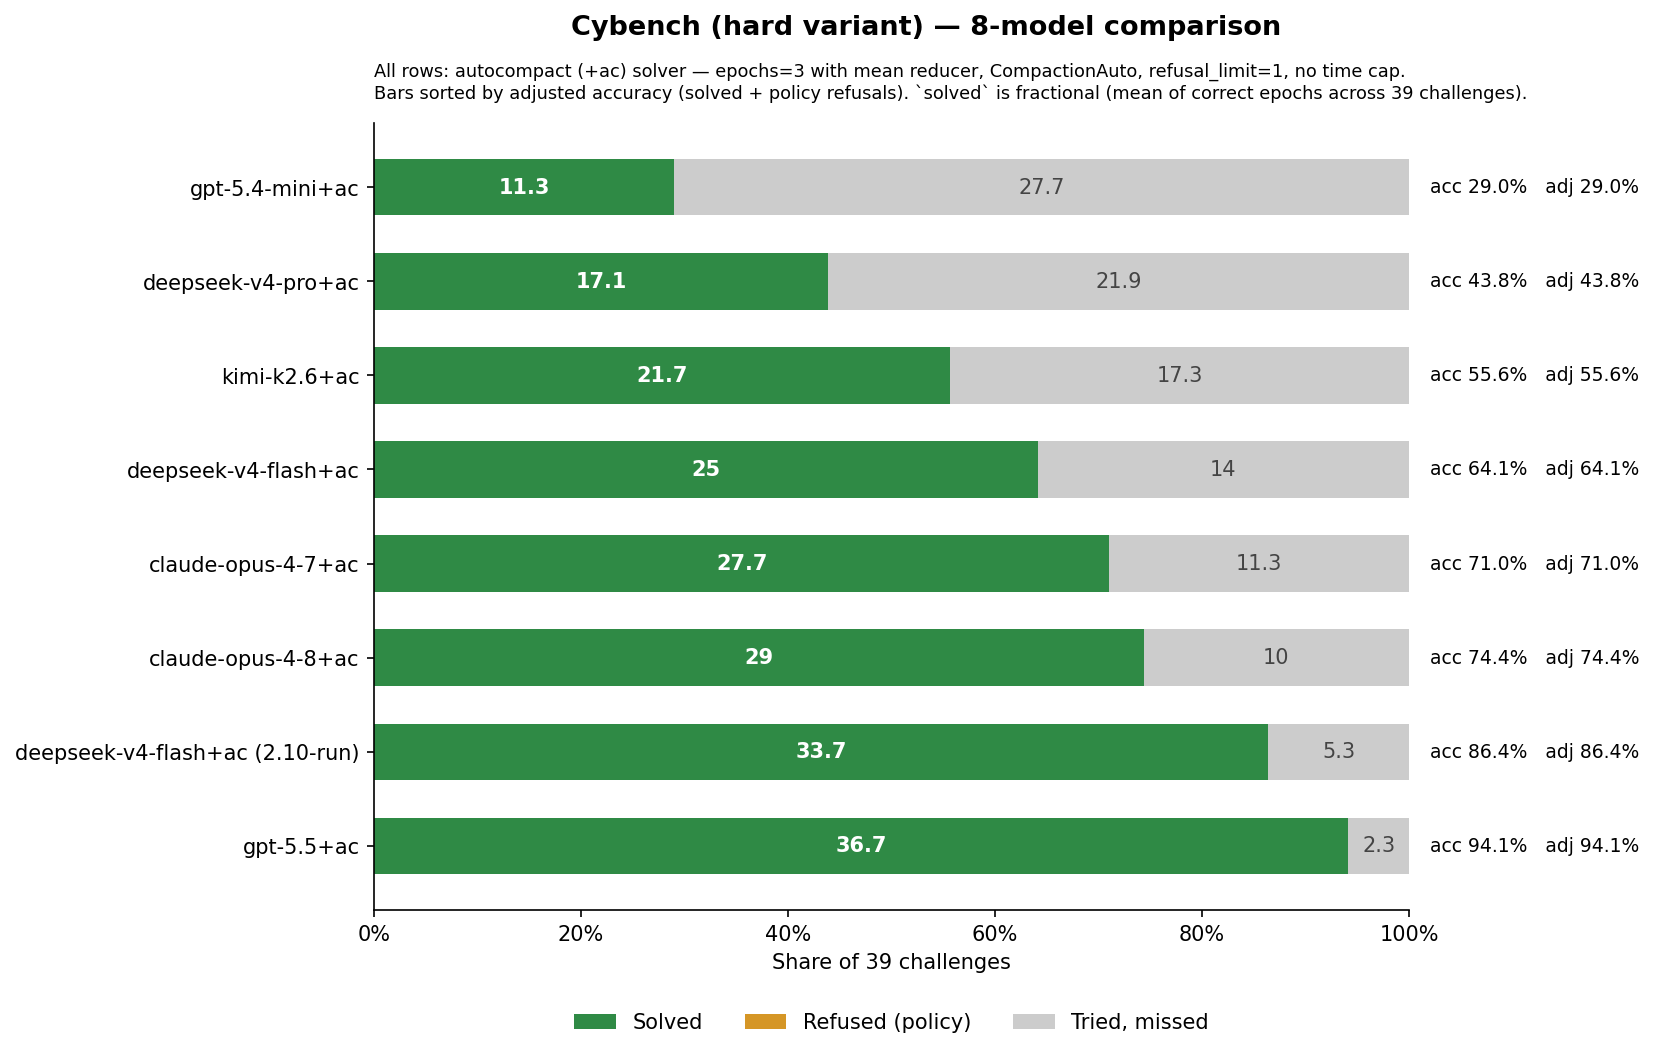
\includegraphics[width=0.95\linewidth]{cybench_comparison.png}
\end{center}
\noindent\textbf{Figure~\thefigure:} Cybench hard-variant comparison generated by source-repository \texttt{charts/make\_report.py}.
\par\medskip

\subsection{BOTSv1: public leaderboard scores require contamination controls}

Table~\ref{tab:bots} gives the BOTSv1 leaderboard.  Claude Opus 4.8 leads by BOTS points: 9,666.7 of 10,300 possible points (93.9\%), with 96.8\% binary accuracy.  It is also the most tool-efficient full run in the table: 603 total tool calls across 31 questions and three epochs.  A question-level paired bootstrap over the 31 scored questions puts Claude's margin over the standard GPT-5.5 row at +12.8 percentage points (95\% CI +0.9 to +27.4).  GPT-5.5 reaches about 81\% of points with 1,481--1,580 calls, while DeepSeek v4 Pro and Flash use still more calls and score lower.  Raising DeepSeek v4 Flash's cap from \$2.10 to \$4.20 adds only 91.7 points; its paired bootstrap interval crosses zero, so I treat that budget change as inconclusive rather than a meaningful gain.

\par\medskip
\refstepcounter{table}\label{tab:bots}
\noindent\textbf{Table~\thetable:} BOTSv1 full-run results from \texttt{charts/botsv1\_report.html}.  BOTS points are the primary \texttt{bots\_points} metric with hint penalties; binary accuracy is secondary.
\begin{center}
\resizebox{\linewidth}{!}{%
\begin{tabular}{lrrrrrrr}
\toprule
Model & BOTS points & points & binary acc. & model cost & tool cost & model+tools & tool calls \\
\midrule
Claude Opus 4.8 & 9{,}666.7 / 10{,}300 & 93.9\% & 96.8\% & \$11.81 & \$1.43 & \$13.24 & 603 \\
GPT-5.5 (high effort) & 8{,}383.3 / 10{,}300 & 81.4\% & 91.4\% & \$46.05 & \$2.94 & \$48.98 & 1{,}580 \\
GPT-5.5 & 8{,}345.0 / 10{,}300 & 81.0\% & 90.3\% & \$41.75 & \$5.54 & \$47.28 & 1{,}481 \\
DeepSeek v4 Pro & 8{,}013.3 / 10{,}300 & 77.8\% & 84.9\% & \$46.44 & \$0.48 & \$46.92 & 3{,}363 \\
DeepSeek v4 Flash (\$4.20 cap) & 7{,}610.0 / 10{,}300 & 73.9\% & 81.7\% & \$22.76 & \$0.53 & \$23.29 & 4{,}938 \\
DeepSeek v4 Flash & 7{,}518.3 / 10{,}300 & 73.0\% & 82.8\% & \$21.89 & \$0.64 & \$22.53 & 4{,}450 \\
GPT-5.4 Mini & 2{,}828.3 / 10{,}300 & 27.5\% & 41.9\% & \$18.16 & \$1.63 & \$19.79 & 1{,}693 \\
\bottomrule
\end{tabular}}
\end{center}

Because BOTSv1 is public and old, I ran a single-epoch no-tools probe using a memory-only solver.  No Splunk, web, bash, Python, or other tools were registered, and the logs contain zero tool events.  With the paper's prerequisite context enabled, Claude scored 7,700/10,300 points (74.8\%) and GPT-5.5 scored 6,400/10,300 (62.1\%).  With \texttt{prereq\_context=false}, Claude still scored 5,150 points (50.0\%) and GPT-5.5 scored 5,650 points (54.9\%).  These controls confirm substantial memorization or public-answer leakage; I therefore treat BOTSv1 as a useful harness and cost-accounting case study, not as clean evidence of fresh SOC investigation skill.

\par\medskip
\refstepcounter{figure}\label{fig:bots-decontamination}
\begin{center}
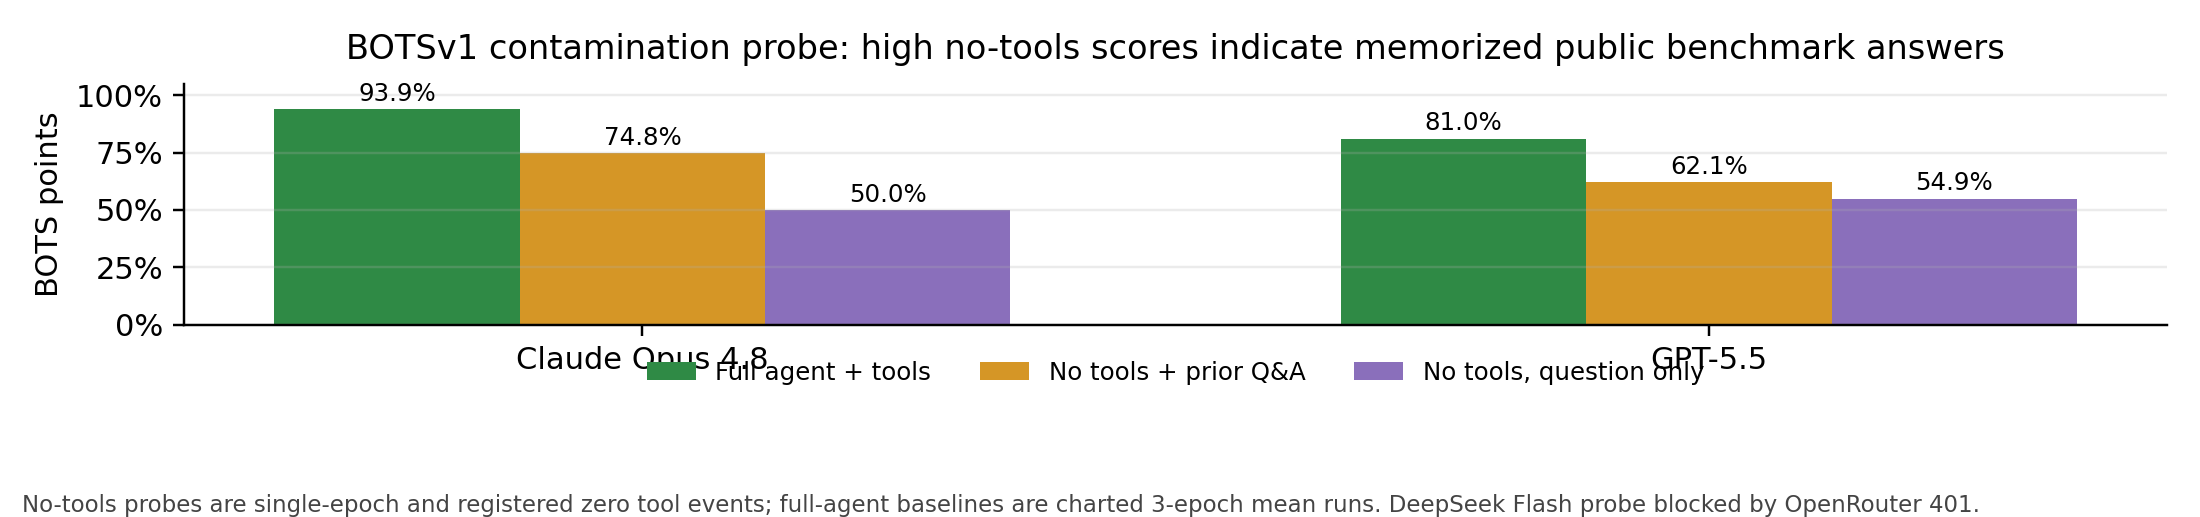
\includegraphics[width=0.95\linewidth]{botsv1_decontamination.png}
\end{center}
\noindent\textbf{Figure~\thefigure:} BOTSv1 no-tools contamination probe.  No-tools rows are single-epoch controls; full-agent baselines are charted three-epoch mean runs.  DeepSeek v4 Flash is omitted because OpenRouter authentication failed before any scored samples completed.
\par\medskip

\section{Discussion and Limitations}

\paragraph{Do not extrapolate SOC readiness from CTF results.}  Cybench is valuable because it measures autonomous challenge solving in realistic sandboxes, but its task shape is closer to offensive exploitation and reverse engineering than to SOC work.  BOTS asks for log-schema discovery, SPL query formulation, hypothesis pruning, external enrichment, and answer formatting under a point-and-hint economy.  The model ordering and resource behavior differ across these task families, so organizations selecting a model for security operations should evaluate on SOC-native workloads; for public SOC benchmarks, they should also run no-tools or perturbed-question controls.

\paragraph{Compute scaling and tool scaling differ by task family.}  The DeepSeek v4 Flash Cybench ablation is evidence that additional per-sample budget can unlock offensive solves.  The analogous BOTSv1 budget increase yields only a small point gain.  In these logs, full-agent defensive performance is associated less with brute-force tool volume than with targeted use of high-quality tools and evidence, but the no-tools controls show that this mechanism cannot be isolated cleanly on public BOTSv1 alone.

\paragraph{Cost accounting changes the question.}  In offensive CTFs, model-token spend is often the dominant marginal cost.  In SOC workflows, external data providers can be part of the real marginal cost of analysis.  Reporting model cost, tool cost, and combined cost makes this tradeoff visible, even though the values here exclude Kubernetes/Splunk infrastructure, free-tier effects, and any enterprise pricing variation.

\paragraph{Limitations.}  The experiments are not a randomized, controlled model-only benchmark.  Cybench rows differ in cost limits, routing, concurrency, sandbox backend, retry-chain cost ledgers, and one challenge-set denominator.  BOTSv1 rows are more uniform at the task level, but provider defaults and reasoning settings still differ.  Bootstrap intervals are descriptive robustness checks, not formal claims of population-level significance.  The defensive analysis covers BOTSv1 only; other SOC datasets and BOTS versions differ in scenario and operational maturity.  The no-tools probes confirm that BOTSv1 absolute scores are contamination-sensitive, and external-enrichment drift remains a separate threat to validity.

\section{Ethics, Artifacts, and Conclusion}

The experiments use public cybersecurity benchmarks and sandboxed environments.  The paper does not publish raw transcripts, secrets, API keys, or exploit instructions beyond high-level benchmark descriptions.  A sanitized supplement can provide aggregate provenance, uncertainty calculations, exact commands, commit hashes, model/provider identifiers, and cost-accounting details without releasing private logs or credentials.

The central finding is simple: security tasks should not be collapsed into one scalar capability.  Offensive CTF benchmarks and defensive SOC investigations stress different agent behaviors and show different scaling patterns, but public SOC benchmarks also need decontamination controls.  Evaluation programs should therefore report task-family-specific results, use scoring that matches the real workflow, account for model and external-tool costs, and test whether agents can answer without evidence tools.  For SOC adoption in particular, the right benchmark is not only ``can the model solve CTFs?'' but ``can the model investigate incidents like an analyst?''

\ifanonymousreview
\else
\section*{Acknowledgments}

Thanks to the maintainers of Inspect, Inspect Evals, Cybench, and Splunk's public BOTS datasets.
\fi

{\small
\bibliographystyle{plainnat}
\bibliography{references}
}

\end{document}
 to build a double-blind
% submission copy, e.g. via `make paper-anonymous`.
\newif\ifanonymousreview
\ifdefined\anonymous
  \anonymousreviewtrue
\else
  \anonymousreviewfalse
\fi

\ifanonymousreview
  \newcommand{\paperauthor}{Anonymous Author(s)}
  \newcommand{\paperaffiliation}{Affiliation(s) withheld for review}
  \newcommand{\paperdate}{Short Paper Submission}
\else
  \newcommand{\paperauthor}{Paul Kassianik}
  \newcommand{\paperaffiliation}{Stealth Company}
  \newcommand{\paperdate}{Short Paper Submission\\\today}
\fi

\title{Offensive CTFs and SOC Investigations Stress Different Agent Behaviors}

\author{
  \paperauthor\\
  \paperaffiliation
}

\date{\paperdate}

\renewcommand{\headeright}{Short Paper Submission}
\renewcommand{\undertitle}{Short Paper Submission}
\renewcommand{\shorttitle}{Offensive and Defensive Agent Evaluation}

\hypersetup{
  pdftitle={Offensive CTFs and SOC Investigations Stress Different Agent Behaviors},
  pdfsubject={Cybersecurity benchmark evaluation},
  pdfauthor={\paperauthor},
  pdfkeywords={cybersecurity benchmarks, AI agents, Cybench, BOTS, Inspect, SOC}
}

\begin{document}
\maketitle

\begin{abstract}
AI security evaluations often emphasize exploit-finding, application-security, or capture-the-flag tasks, while security operations center (SOC) work asks whether an agent can navigate telemetry, pivot through evidence, and spend enrichment calls with analyst discipline.  I report Inspect-based experiments on two public benchmark families: Cybench hard-variant CTF challenges and Splunk Boss of the SOC (BOTS) v1 investigations.  The results do not support a single universal model ranking.  On Cybench, GPT-5.5 reached 94.1\% pass@1; DeepSeek v4 Flash improved from 64.1\% to 86.4\% when its per-sample budget was raised; and Claude Opus 4.8 reached 74.4\%, below those two rows despite leading BOTSv1.  On BOTSv1, Claude Opus 4.8 earned 9,666.7/10,300 competition points (93.9\%) with 603 tool calls and \$13.24 in model-plus-priced-tool spend, while GPT-5.5 earned about 81\% of points with more than twice the tool calls and over three times the cost.  However, no-tools BOTSv1 probes still scored 74.8\% for Claude and 62.1\% for GPT-5.5 with prerequisite context, confirming substantial public-benchmark contamination.  These findings argue for SOC-native agent benchmarks with workflow-appropriate scoring, cost accounting, and decontamination controls.
\end{abstract}

\keywords{cybersecurity benchmarks \and AI agents \and SOC \and Cybench \and BOTS \and Inspect}

\section{Introduction}

The current discussion of AI for security is shaped by application-security demonstrations: models find bugs, reason about code, and sometimes exploit vulnerable services.  Those capabilities matter, but they do not exhaust the work of security teams.  Incident-response guidance and cybersecurity workforce taxonomies emphasize detection, analysis, evidence handling, and response coordination as distinct work from vulnerability discovery \citep{nist_sp800_61r3,nist_nice_800_181r1}.  A SOC analyst spends much of a shift formulating searches over telemetry, validating weak signals, correlating host/network/application evidence, and deciding when external enrichment is worth its cost and latency.

This short paper compares offensive and defensive agent behavior using a local Inspect \citep{inspect_ai_2024} harness.  Cybench \citep{zhang2024cybench,inspect_evals_cybench} represents offensive, CTF-style tasks: agents work in challenge sandboxes with shell/Python tools and submit flags.  Splunk Boss of the SOC (BOTS) v1 \citep{splunk_botsv1} represents defensive investigation: agents answer forensic questions over Splunk telemetry, with competition points and hint penalties.  The contribution is not a definitive procurement leaderboard.  The charted rows differ in some model/provider settings, cost limits, routing, and concurrency.  Instead, the paper contributes:

\begin{itemize}
  \item a task-family comparison showing that CTF and SOC investigations stress different agent behaviors;
  \item a cost-aware BOTSv1 analysis that includes priced external enrichment calls, not only model-token spend;
  \item practical evaluation guidance: report SOC results with SOC-native tools, scoring, provenance, decontamination controls, and caveats.
\end{itemize}

\section{Related Work}

Recent LLM cyber evaluations cover broad risk and capability suites, interactive coding, CTF-like tasks, and exploit-oriented web-application settings \citep{bhatt2024cyberseceval2,yang2023intercode,yang2023languagehackers,zhu2025cvebench}.  Cybench extends this line with professional CTF tasks in sandboxed environments \citep{zhang2024cybench}.  This paper uses Cybench as an offensive comparison point and focuses the defensive side on public SOC data from Splunk BOTS.  The distinction matters because SOC investigation is not simply exploitation with different labels: it asks for log-schema discovery, SPL formulation, hypothesis pruning, historical context, and cost-sensitive enrichment.

\section{Benchmarks and Methodology}

All quantitative claims were checked against the source evaluation repository: generated chart tables/reports under \path{charts/} and raw Inspect logs under \path{logs/}.  The analysis is descriptive rather than a randomized model-only benchmark.  To avoid overstating close differences, I bootstrap at the task granularity: Cybench resamples challenges while retaining their three epochs, and BOTSv1 resamples questions while retaining their three epochs and point weights.

\paragraph{Cybench.}  The charted ``+ac'' rows use \texttt{inspect\_evals/cybench} hard variant, mostly with Docker sandboxes; the Claude Opus 4.8 row used a Kubernetes sandbox to avoid local Docker subnet exhaustion.  All use \path{agents/react_autocompact.py@react_autocompact}, bash/Python tools with 180-second timeouts, a three-attempt ReAct loop \citep{yao2023react}, Inspect automatic compaction, and a one-refusal abort rule.  Runs use three epochs and a mean reducer.  The headline metric is upstream \texttt{includes} accuracy; ``solved'' is the mean-correct equivalent out of 39 challenges.

\paragraph{BOTSv1.}  This paper reports the complete audited BOTSv1 comparison: official warm-up question 1 is excluded, leaving 31 scored questions; each run uses three epochs, a mean reducer, message limit 250, and a Kubernetes sandbox (\texttt{chart} or \texttt{chart-bots-data-2}, depending on row).  Because BOTSv1 is sequential, prompts include prerequisite context for dependent questions; 23 of 31 scored questions have such dependencies, so the task measures incident follow-up with known case state rather than cold-start reconstruction.  Agents receive Splunk discovery/search/event tools, limited VirusTotal/WHOIS/DNS/Brave enrichment, and guarded bash/Python tools.  The primary scorer is \texttt{bots\_points}: a correct answer earns \(\max(0,\text{base points}-\text{hint penalty})\), while an incorrect answer earns 0.  Binary \texttt{includes} accuracy is secondary.

\paragraph{Cost accounting and caveats.}  Cybench costs are model-token costs from Inspect's usage ledger or reconstructed from token counts when provider APIs did not populate \texttt{total\_cost}.  BOTSv1 costs add priced external enrichment calls visible in transcripts: Brave Search at \$0.005/request and non-cache WhoisXMLAPI WHOIS History credits converted at \$129/5,000 credits.  VirusTotal public API, DNS, and live WHOIS/RDAP are treated as zero marginal cost.  The runs are not a fully controlled model-only experiment: cost limits, OpenRouter routing, concurrency, and some provider defaults differ; DeepSeek v4 Pro on Cybench used 38 challenges because one challenge had a deterministic sandbox initialization failure.

\section{Results}

\subsection{Cybench: additional budget can buy offensive progress}

Table~\ref{tab:cybench} summarizes the charted Cybench rows.  GPT-5.5 is the top row at 94.1\% pass@1.  The cleanest budget signal is DeepSeek v4 Flash: raising the per-sample cap from \$0.80 to \$2.10 moved pass@1 from 64.1\% to 86.4\%, or from 25.0 to 33.7 solved-equivalent challenges.  Claude Opus 4.8 reached 74.4\% (29.0 solved-equivalent challenges), ahead of Opus 4.7 but still below GPT-5.5 and the higher-budget DeepSeek v4 Flash row.  A challenge-level paired bootstrap estimates the DeepSeek budget effect at +22.2 percentage points (95\% CI +12.8 to +32.5).  Tool volume alone did not explain success: GPT-5.5 solved more with a mean of 20.6 non-submit tool events per sample epoch, while the higher-budget DeepSeek v4 Flash run averaged 144.7.

\par\medskip
\refstepcounter{table}\label{tab:cybench}
\noindent\textbf{Table~\thetable:} Cybench hard-variant results from \texttt{charts/cybench\_cost\_table.csv}, \texttt{charts/cybench\_report.html}, and raw logs.  DeepSeek v4 Pro used 38 challenges; its solved value follows the generated chart's 39-challenge normalization.
\begin{center}
\resizebox{\linewidth}{!}{%
\begin{tabular}{lrrrrrr}
\toprule
Model & pass@1 & solved & refused & run cost & \$/solve & mean tool calls \\
\midrule
GPT-5.5 + autocompact & 94.1\% & 36.7 & 0.0\% & \$42.47 & \$1.16 & 20.6 \\
DeepSeek v4 Flash + autocompact (\$2.10 cap) & 86.4\% & 33.7 & 0.0\% & \$48.88 & \$1.45 & 144.7 \\
Claude Opus 4.8 + autocompact & 74.4\% & 29.0 & 0.0\% & \$108.21 & \$3.73 & 26.7 \\
Claude Opus 4.7 + autocompact & 71.0\% & 27.7 & 0.0\% & \$92.75 & \$3.35 & 19.7 \\
DeepSeek v4 Flash + autocompact (\$0.80 cap) & 64.1\% & 25.0 & 0.0\% & \$43.09 & \$1.72 & 65.4 \\
Kimi K2.6 + autocompact & 55.6\% & 21.7 & 0.0\% & \$58.55 & \$2.70 & 38.1 \\
DeepSeek v4 Pro + autocompact & 43.8\% & 17.1 & 0.0\% & \$64.58 & \$3.78 & 21.3 \\
GPT-5.4 Mini + autocompact & 29.0\% & 11.3 & 60.7\% & \$13.77 & \$1.22 & 20.9 \\
\bottomrule
\end{tabular}}
\end{center}

\par\medskip
\refstepcounter{figure}\label{fig:cybench-comparison}
\begin{center}
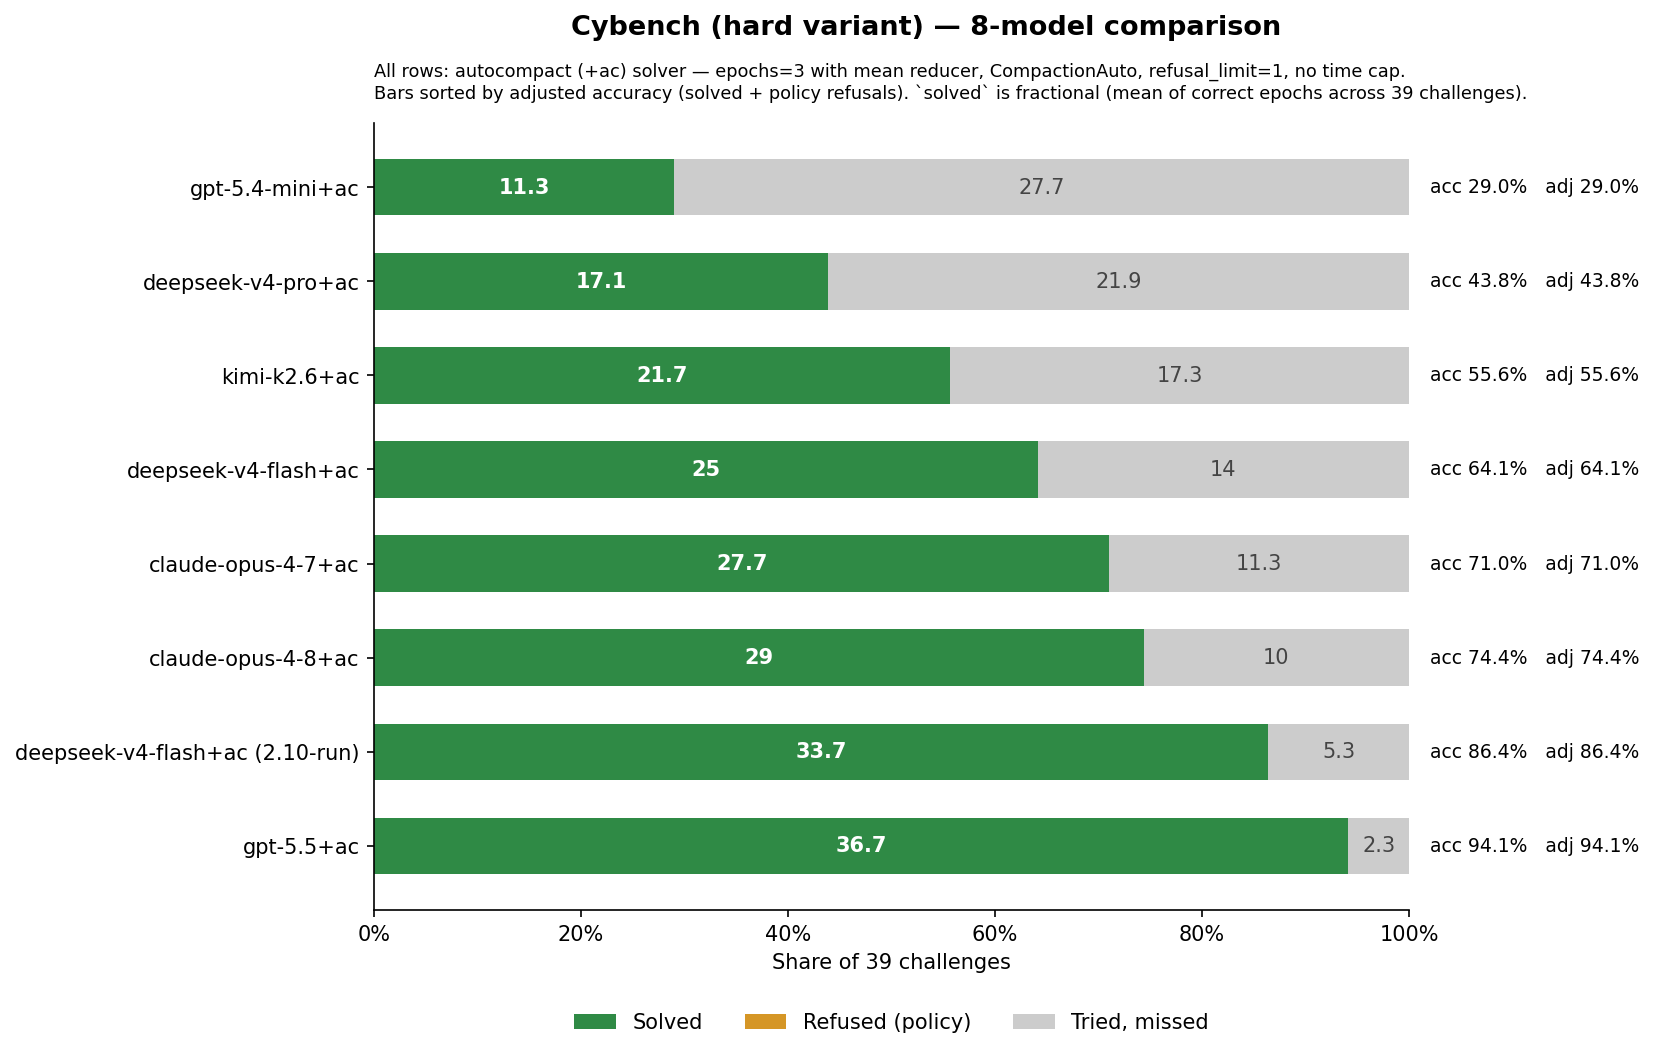
\includegraphics[width=0.95\linewidth]{cybench_comparison.png}
\end{center}
\noindent\textbf{Figure~\thefigure:} Cybench hard-variant comparison generated by source-repository \texttt{charts/make\_report.py}.
\par\medskip

\subsection{BOTSv1: public leaderboard scores require contamination controls}

Table~\ref{tab:bots} gives the BOTSv1 leaderboard.  Claude Opus 4.8 leads by BOTS points: 9,666.7 of 10,300 possible points (93.9\%), with 96.8\% binary accuracy.  It is also the most tool-efficient full run in the table: 603 total tool calls across 31 questions and three epochs.  A question-level paired bootstrap over the 31 scored questions puts Claude's margin over the standard GPT-5.5 row at +12.8 percentage points (95\% CI +0.9 to +27.4).  GPT-5.5 reaches about 81\% of points with 1,481--1,580 calls, while DeepSeek v4 Pro and Flash use still more calls and score lower.  Raising DeepSeek v4 Flash's cap from \$2.10 to \$4.20 adds only 91.7 points; its paired bootstrap interval crosses zero, so I treat that budget change as inconclusive rather than a meaningful gain.

\par\medskip
\refstepcounter{table}\label{tab:bots}
\noindent\textbf{Table~\thetable:} BOTSv1 full-run results from \texttt{charts/botsv1\_report.html}.  BOTS points are the primary \texttt{bots\_points} metric with hint penalties; binary accuracy is secondary.
\begin{center}
\resizebox{\linewidth}{!}{%
\begin{tabular}{lrrrrrrr}
\toprule
Model & BOTS points & points & binary acc. & model cost & tool cost & model+tools & tool calls \\
\midrule
Claude Opus 4.8 & 9{,}666.7 / 10{,}300 & 93.9\% & 96.8\% & \$11.81 & \$1.43 & \$13.24 & 603 \\
GPT-5.5 (high effort) & 8{,}383.3 / 10{,}300 & 81.4\% & 91.4\% & \$46.05 & \$2.94 & \$48.98 & 1{,}580 \\
GPT-5.5 & 8{,}345.0 / 10{,}300 & 81.0\% & 90.3\% & \$41.75 & \$5.54 & \$47.28 & 1{,}481 \\
DeepSeek v4 Pro & 8{,}013.3 / 10{,}300 & 77.8\% & 84.9\% & \$46.44 & \$0.48 & \$46.92 & 3{,}363 \\
DeepSeek v4 Flash (\$4.20 cap) & 7{,}610.0 / 10{,}300 & 73.9\% & 81.7\% & \$22.76 & \$0.53 & \$23.29 & 4{,}938 \\
DeepSeek v4 Flash & 7{,}518.3 / 10{,}300 & 73.0\% & 82.8\% & \$21.89 & \$0.64 & \$22.53 & 4{,}450 \\
GPT-5.4 Mini & 2{,}828.3 / 10{,}300 & 27.5\% & 41.9\% & \$18.16 & \$1.63 & \$19.79 & 1{,}693 \\
\bottomrule
\end{tabular}}
\end{center}

Because BOTSv1 is public and old, I ran a single-epoch no-tools probe using a memory-only solver.  No Splunk, web, bash, Python, or other tools were registered, and the logs contain zero tool events.  With the paper's prerequisite context enabled, Claude scored 7,700/10,300 points (74.8\%) and GPT-5.5 scored 6,400/10,300 (62.1\%).  With \texttt{prereq\_context=false}, Claude still scored 5,150 points (50.0\%) and GPT-5.5 scored 5,650 points (54.9\%).  These controls confirm substantial memorization or public-answer leakage; I therefore treat BOTSv1 as a useful harness and cost-accounting case study, not as clean evidence of fresh SOC investigation skill.

\par\medskip
\refstepcounter{figure}\label{fig:bots-decontamination}
\begin{center}
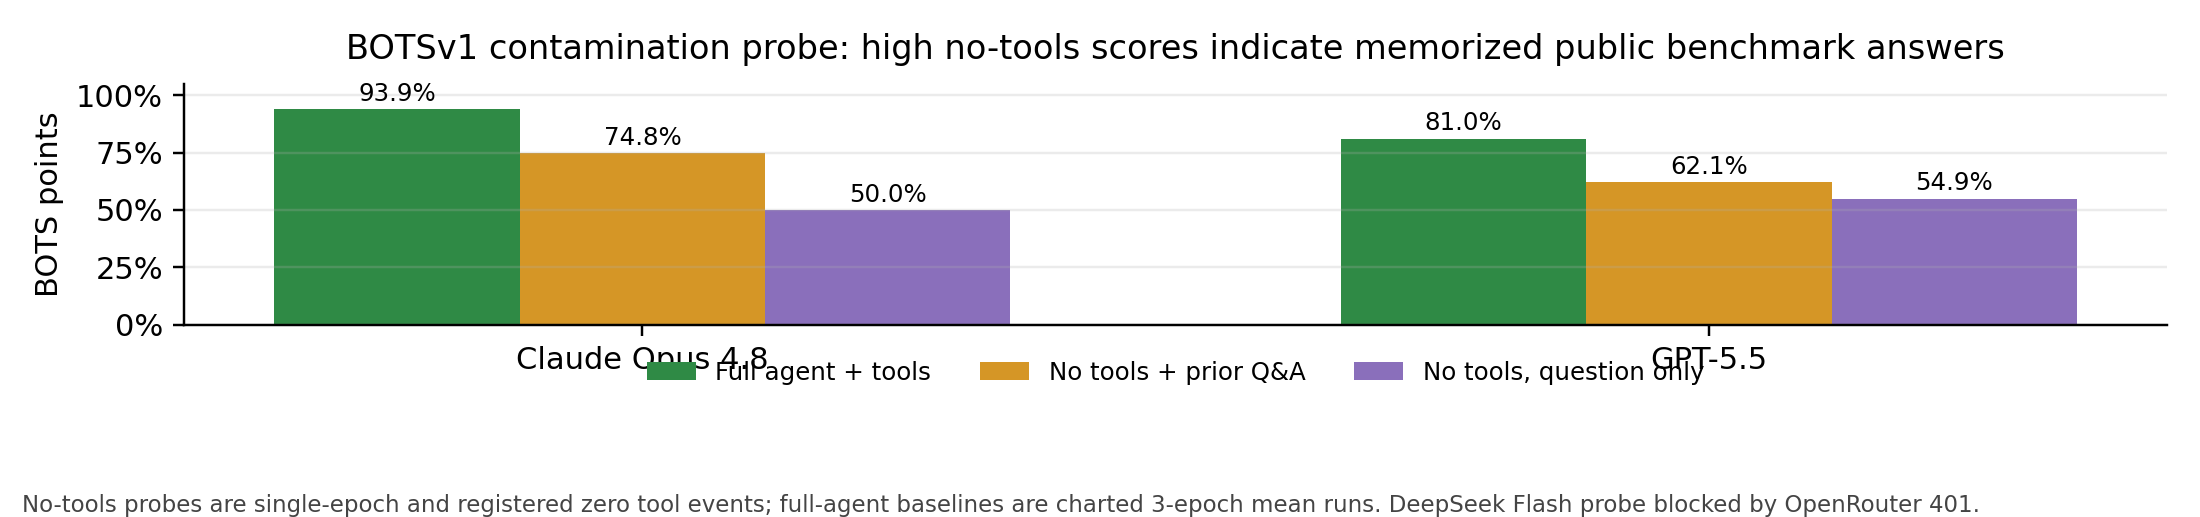
\includegraphics[width=0.95\linewidth]{botsv1_decontamination.png}
\end{center}
\noindent\textbf{Figure~\thefigure:} BOTSv1 no-tools contamination probe.  No-tools rows are single-epoch controls; full-agent baselines are charted three-epoch mean runs.  DeepSeek v4 Flash is omitted because OpenRouter authentication failed before any scored samples completed.
\par\medskip

\section{Discussion and Limitations}

\paragraph{Do not extrapolate SOC readiness from CTF results.}  Cybench is valuable because it measures autonomous challenge solving in realistic sandboxes, but its task shape is closer to offensive exploitation and reverse engineering than to SOC work.  BOTS asks for log-schema discovery, SPL query formulation, hypothesis pruning, external enrichment, and answer formatting under a point-and-hint economy.  The model ordering and resource behavior differ across these task families, so organizations selecting a model for security operations should evaluate on SOC-native workloads; for public SOC benchmarks, they should also run no-tools or perturbed-question controls.

\paragraph{Compute scaling and tool scaling differ by task family.}  The DeepSeek v4 Flash Cybench ablation is evidence that additional per-sample budget can unlock offensive solves.  The analogous BOTSv1 budget increase yields only a small point gain.  In these logs, full-agent defensive performance is associated less with brute-force tool volume than with targeted use of high-quality tools and evidence, but the no-tools controls show that this mechanism cannot be isolated cleanly on public BOTSv1 alone.

\paragraph{Cost accounting changes the question.}  In offensive CTFs, model-token spend is often the dominant marginal cost.  In SOC workflows, external data providers can be part of the real marginal cost of analysis.  Reporting model cost, tool cost, and combined cost makes this tradeoff visible, even though the values here exclude Kubernetes/Splunk infrastructure, free-tier effects, and any enterprise pricing variation.

\paragraph{Limitations.}  The experiments are not a randomized, controlled model-only benchmark.  Cybench rows differ in cost limits, routing, concurrency, sandbox backend, retry-chain cost ledgers, and one challenge-set denominator.  BOTSv1 rows are more uniform at the task level, but provider defaults and reasoning settings still differ.  Bootstrap intervals are descriptive robustness checks, not formal claims of population-level significance.  The defensive analysis covers BOTSv1 only; other SOC datasets and BOTS versions differ in scenario and operational maturity.  The no-tools probes confirm that BOTSv1 absolute scores are contamination-sensitive, and external-enrichment drift remains a separate threat to validity.

\section{Ethics, Artifacts, and Conclusion}

The experiments use public cybersecurity benchmarks and sandboxed environments.  The paper does not publish raw transcripts, secrets, API keys, or exploit instructions beyond high-level benchmark descriptions.  A sanitized supplement can provide aggregate provenance, uncertainty calculations, exact commands, commit hashes, model/provider identifiers, and cost-accounting details without releasing private logs or credentials.

The central finding is simple: security tasks should not be collapsed into one scalar capability.  Offensive CTF benchmarks and defensive SOC investigations stress different agent behaviors and show different scaling patterns, but public SOC benchmarks also need decontamination controls.  Evaluation programs should therefore report task-family-specific results, use scoring that matches the real workflow, account for model and external-tool costs, and test whether agents can answer without evidence tools.  For SOC adoption in particular, the right benchmark is not only ``can the model solve CTFs?'' but ``can the model investigate incidents like an analyst?''

\ifanonymousreview
\else
\section*{Acknowledgments}

Thanks to the maintainers of Inspect, Inspect Evals, Cybench, and Splunk's public BOTS datasets.
\fi

{\small
\bibliographystyle{plainnat}
\bibliography{references}
}

\end{document}
 to build a double-blind
% submission copy, e.g. via `make paper-anonymous`.
\newif\ifanonymousreview
\ifdefined\anonymous
  \anonymousreviewtrue
\else
  \anonymousreviewfalse
\fi

\ifanonymousreview
  \newcommand{\paperauthor}{Anonymous Author(s)}
  \newcommand{\paperaffiliation}{Affiliation(s) withheld for review}
  \newcommand{\paperdate}{Short Paper Submission}
\else
  \newcommand{\paperauthor}{Paul Kassianik}
  \newcommand{\paperaffiliation}{Stealth Company}
  \newcommand{\paperdate}{Short Paper Submission\\\today}
\fi

\title{Offensive CTFs and SOC Investigations Stress Different Agent Behaviors}

\author{
  \paperauthor\\
  \paperaffiliation
}

\date{\paperdate}

\renewcommand{\headeright}{Short Paper Submission}
\renewcommand{\undertitle}{Short Paper Submission}
\renewcommand{\shorttitle}{Offensive and Defensive Agent Evaluation}

\hypersetup{
  pdftitle={Offensive CTFs and SOC Investigations Stress Different Agent Behaviors},
  pdfsubject={Cybersecurity benchmark evaluation},
  pdfauthor={\paperauthor},
  pdfkeywords={cybersecurity benchmarks, AI agents, Cybench, BOTS, Inspect, SOC}
}

\begin{document}
\maketitle

\begin{abstract}
AI security evaluations often emphasize exploit-finding, application-security, or capture-the-flag tasks, while security operations center (SOC) work asks whether an agent can navigate telemetry, pivot through evidence, and spend enrichment calls with analyst discipline.  I report Inspect-based experiments on two public benchmark families: Cybench hard-variant CTF challenges and Splunk Boss of the SOC (BOTS) v1 investigations.  The results do not support a single universal model ranking.  On Cybench, GPT-5.5 reached 94.1\% pass@1; DeepSeek v4 Flash improved from 64.1\% to 86.4\% when its per-sample budget was raised; and Claude Opus 4.8 reached 74.4\%, below those two rows despite leading BOTSv1.  On BOTSv1, Claude Opus 4.8 earned 9,666.7/10,300 competition points (93.9\%) with 603 tool calls and \$13.24 in model-plus-priced-tool spend, while GPT-5.5 earned about 81\% of points with more than twice the tool calls and over three times the cost.  However, no-tools BOTSv1 probes still scored 74.8\% for Claude and 62.1\% for GPT-5.5 with prerequisite context, confirming substantial public-benchmark contamination.  These findings argue for SOC-native agent benchmarks with workflow-appropriate scoring, cost accounting, and decontamination controls.
\end{abstract}

\keywords{cybersecurity benchmarks \and AI agents \and SOC \and Cybench \and BOTS \and Inspect}

\section{Introduction}

The current discussion of AI for security is shaped by application-security demonstrations: models find bugs, reason about code, and sometimes exploit vulnerable services.  Those capabilities matter, but they do not exhaust the work of security teams.  Incident-response guidance and cybersecurity workforce taxonomies emphasize detection, analysis, evidence handling, and response coordination as distinct work from vulnerability discovery \citep{nist_sp800_61r3,nist_nice_800_181r1}.  A SOC analyst spends much of a shift formulating searches over telemetry, validating weak signals, correlating host/network/application evidence, and deciding when external enrichment is worth its cost and latency.

This short paper compares offensive and defensive agent behavior using a local Inspect \citep{inspect_ai_2024} harness.  Cybench \citep{zhang2024cybench,inspect_evals_cybench} represents offensive, CTF-style tasks: agents work in challenge sandboxes with shell/Python tools and submit flags.  Splunk Boss of the SOC (BOTS) v1 \citep{splunk_botsv1} represents defensive investigation: agents answer forensic questions over Splunk telemetry, with competition points and hint penalties.  The contribution is not a definitive procurement leaderboard.  The charted rows differ in some model/provider settings, cost limits, routing, and concurrency.  Instead, the paper contributes:

\begin{itemize}
  \item a task-family comparison showing that CTF and SOC investigations stress different agent behaviors;
  \item a cost-aware BOTSv1 analysis that includes priced external enrichment calls, not only model-token spend;
  \item practical evaluation guidance: report SOC results with SOC-native tools, scoring, provenance, decontamination controls, and caveats.
\end{itemize}

\section{Related Work}

Recent LLM cyber evaluations cover broad risk and capability suites, interactive coding, CTF-like tasks, and exploit-oriented web-application settings \citep{bhatt2024cyberseceval2,yang2023intercode,yang2023languagehackers,zhu2025cvebench}.  Cybench extends this line with professional CTF tasks in sandboxed environments \citep{zhang2024cybench}.  This paper uses Cybench as an offensive comparison point and focuses the defensive side on public SOC data from Splunk BOTS.  The distinction matters because SOC investigation is not simply exploitation with different labels: it asks for log-schema discovery, SPL formulation, hypothesis pruning, historical context, and cost-sensitive enrichment.

\section{Benchmarks and Methodology}

All quantitative claims were checked against the source evaluation repository: generated chart tables/reports under \path{charts/} and raw Inspect logs under \path{logs/}.  The analysis is descriptive rather than a randomized model-only benchmark.  To avoid overstating close differences, I bootstrap at the task granularity: Cybench resamples challenges while retaining their three epochs, and BOTSv1 resamples questions while retaining their three epochs and point weights.

\paragraph{Cybench.}  The charted ``+ac'' rows use \texttt{inspect\_evals/cybench} hard variant, mostly with Docker sandboxes; the Claude Opus 4.8 row used a Kubernetes sandbox to avoid local Docker subnet exhaustion.  All use \path{agents/react_autocompact.py@react_autocompact}, bash/Python tools with 180-second timeouts, a three-attempt ReAct loop \citep{yao2023react}, Inspect automatic compaction, and a one-refusal abort rule.  Runs use three epochs and a mean reducer.  The headline metric is upstream \texttt{includes} accuracy; ``solved'' is the mean-correct equivalent out of 39 challenges.

\paragraph{BOTSv1.}  This paper reports the complete audited BOTSv1 comparison: official warm-up question 1 is excluded, leaving 31 scored questions; each run uses three epochs, a mean reducer, message limit 250, and a Kubernetes sandbox (\texttt{chart} or \texttt{chart-bots-data-2}, depending on row).  Because BOTSv1 is sequential, prompts include prerequisite context for dependent questions; 23 of 31 scored questions have such dependencies, so the task measures incident follow-up with known case state rather than cold-start reconstruction.  Agents receive Splunk discovery/search/event tools, limited VirusTotal/WHOIS/DNS/Brave enrichment, and guarded bash/Python tools.  The primary scorer is \texttt{bots\_points}: a correct answer earns \(\max(0,\text{base points}-\text{hint penalty})\), while an incorrect answer earns 0.  Binary \texttt{includes} accuracy is secondary.

\paragraph{Cost accounting and caveats.}  Cybench costs are model-token costs from Inspect's usage ledger or reconstructed from token counts when provider APIs did not populate \texttt{total\_cost}.  BOTSv1 costs add priced external enrichment calls visible in transcripts: Brave Search at \$0.005/request and non-cache WhoisXMLAPI WHOIS History credits converted at \$129/5,000 credits.  VirusTotal public API, DNS, and live WHOIS/RDAP are treated as zero marginal cost.  The runs are not a fully controlled model-only experiment: cost limits, OpenRouter routing, concurrency, and some provider defaults differ; DeepSeek v4 Pro on Cybench used 38 challenges because one challenge had a deterministic sandbox initialization failure.

\section{Results}

\subsection{Cybench: additional budget can buy offensive progress}

Table~\ref{tab:cybench} summarizes the charted Cybench rows.  GPT-5.5 is the top row at 94.1\% pass@1.  The cleanest budget signal is DeepSeek v4 Flash: raising the per-sample cap from \$0.80 to \$2.10 moved pass@1 from 64.1\% to 86.4\%, or from 25.0 to 33.7 solved-equivalent challenges.  Claude Opus 4.8 reached 74.4\% (29.0 solved-equivalent challenges), ahead of Opus 4.7 but still below GPT-5.5 and the higher-budget DeepSeek v4 Flash row.  A challenge-level paired bootstrap estimates the DeepSeek budget effect at +22.2 percentage points (95\% CI +12.8 to +32.5).  Tool volume alone did not explain success: GPT-5.5 solved more with a mean of 20.6 non-submit tool events per sample epoch, while the higher-budget DeepSeek v4 Flash run averaged 144.7.

\par\medskip
\refstepcounter{table}\label{tab:cybench}
\noindent\textbf{Table~\thetable:} Cybench hard-variant results from \texttt{charts/cybench\_cost\_table.csv}, \texttt{charts/cybench\_report.html}, and raw logs.  DeepSeek v4 Pro used 38 challenges; its solved value follows the generated chart's 39-challenge normalization.
\begin{center}
\resizebox{\linewidth}{!}{%
\begin{tabular}{lrrrrrr}
\toprule
Model & pass@1 & solved & refused & run cost & \$/solve & mean tool calls \\
\midrule
GPT-5.5 + autocompact & 94.1\% & 36.7 & 0.0\% & \$42.47 & \$1.16 & 20.6 \\
DeepSeek v4 Flash + autocompact (\$2.10 cap) & 86.4\% & 33.7 & 0.0\% & \$48.88 & \$1.45 & 144.7 \\
Claude Opus 4.8 + autocompact & 74.4\% & 29.0 & 0.0\% & \$108.21 & \$3.73 & 26.7 \\
Claude Opus 4.7 + autocompact & 71.0\% & 27.7 & 0.0\% & \$92.75 & \$3.35 & 19.7 \\
DeepSeek v4 Flash + autocompact (\$0.80 cap) & 64.1\% & 25.0 & 0.0\% & \$43.09 & \$1.72 & 65.4 \\
Kimi K2.6 + autocompact & 55.6\% & 21.7 & 0.0\% & \$58.55 & \$2.70 & 38.1 \\
DeepSeek v4 Pro + autocompact & 43.8\% & 17.1 & 0.0\% & \$64.58 & \$3.78 & 21.3 \\
GPT-5.4 Mini + autocompact & 29.0\% & 11.3 & 60.7\% & \$13.77 & \$1.22 & 20.9 \\
\bottomrule
\end{tabular}}
\end{center}

\par\medskip
\refstepcounter{figure}\label{fig:cybench-comparison}
\begin{center}
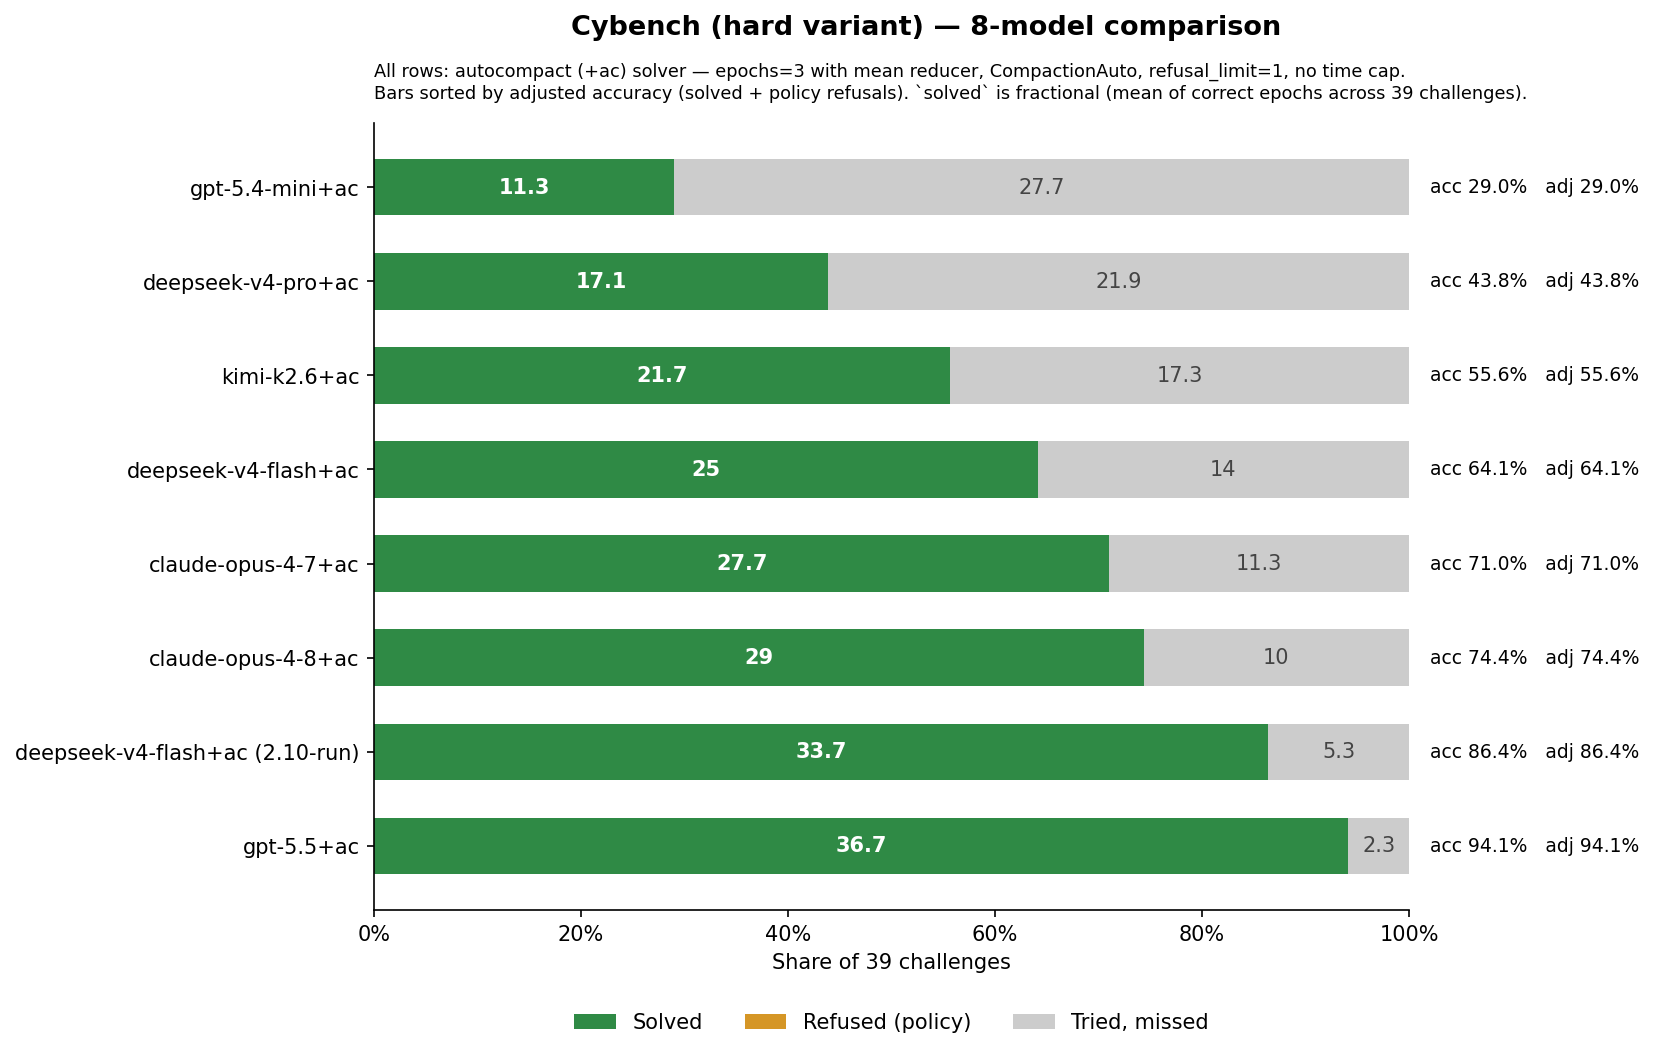
\includegraphics[width=0.95\linewidth]{cybench_comparison.png}
\end{center}
\noindent\textbf{Figure~\thefigure:} Cybench hard-variant comparison generated by source-repository \texttt{charts/make\_report.py}.
\par\medskip

\subsection{BOTSv1: public leaderboard scores require contamination controls}

Table~\ref{tab:bots} gives the BOTSv1 leaderboard.  Claude Opus 4.8 leads by BOTS points: 9,666.7 of 10,300 possible points (93.9\%), with 96.8\% binary accuracy.  It is also the most tool-efficient full run in the table: 603 total tool calls across 31 questions and three epochs.  A question-level paired bootstrap over the 31 scored questions puts Claude's margin over the standard GPT-5.5 row at +12.8 percentage points (95\% CI +0.9 to +27.4).  GPT-5.5 reaches about 81\% of points with 1,481--1,580 calls, while DeepSeek v4 Pro and Flash use still more calls and score lower.  Raising DeepSeek v4 Flash's cap from \$2.10 to \$4.20 adds only 91.7 points; its paired bootstrap interval crosses zero, so I treat that budget change as inconclusive rather than a meaningful gain.

\par\medskip
\refstepcounter{table}\label{tab:bots}
\noindent\textbf{Table~\thetable:} BOTSv1 full-run results from \texttt{charts/botsv1\_report.html}.  BOTS points are the primary \texttt{bots\_points} metric with hint penalties; binary accuracy is secondary.
\begin{center}
\resizebox{\linewidth}{!}{%
\begin{tabular}{lrrrrrrr}
\toprule
Model & BOTS points & points & binary acc. & model cost & tool cost & model+tools & tool calls \\
\midrule
Claude Opus 4.8 & 9{,}666.7 / 10{,}300 & 93.9\% & 96.8\% & \$11.81 & \$1.43 & \$13.24 & 603 \\
GPT-5.5 (high effort) & 8{,}383.3 / 10{,}300 & 81.4\% & 91.4\% & \$46.05 & \$2.94 & \$48.98 & 1{,}580 \\
GPT-5.5 & 8{,}345.0 / 10{,}300 & 81.0\% & 90.3\% & \$41.75 & \$5.54 & \$47.28 & 1{,}481 \\
DeepSeek v4 Pro & 8{,}013.3 / 10{,}300 & 77.8\% & 84.9\% & \$46.44 & \$0.48 & \$46.92 & 3{,}363 \\
DeepSeek v4 Flash (\$4.20 cap) & 7{,}610.0 / 10{,}300 & 73.9\% & 81.7\% & \$22.76 & \$0.53 & \$23.29 & 4{,}938 \\
DeepSeek v4 Flash & 7{,}518.3 / 10{,}300 & 73.0\% & 82.8\% & \$21.89 & \$0.64 & \$22.53 & 4{,}450 \\
GPT-5.4 Mini & 2{,}828.3 / 10{,}300 & 27.5\% & 41.9\% & \$18.16 & \$1.63 & \$19.79 & 1{,}693 \\
\bottomrule
\end{tabular}}
\end{center}

Because BOTSv1 is public and old, I ran a single-epoch no-tools probe using a memory-only solver.  No Splunk, web, bash, Python, or other tools were registered, and the logs contain zero tool events.  With the paper's prerequisite context enabled, Claude scored 7,700/10,300 points (74.8\%) and GPT-5.5 scored 6,400/10,300 (62.1\%).  With \texttt{prereq\_context=false}, Claude still scored 5,150 points (50.0\%) and GPT-5.5 scored 5,650 points (54.9\%).  These controls confirm substantial memorization or public-answer leakage; I therefore treat BOTSv1 as a useful harness and cost-accounting case study, not as clean evidence of fresh SOC investigation skill.

\par\medskip
\refstepcounter{figure}\label{fig:bots-decontamination}
\begin{center}
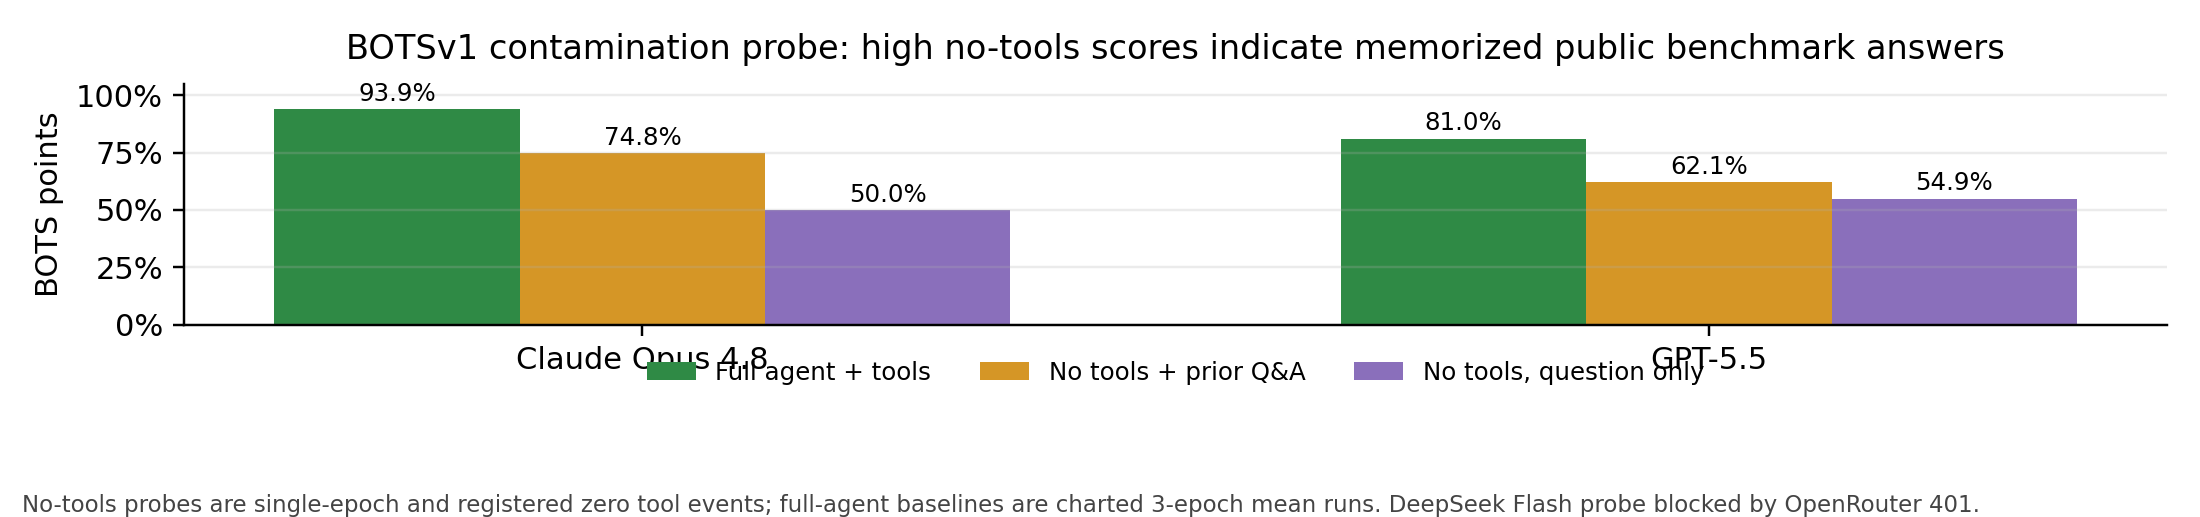
\includegraphics[width=0.95\linewidth]{botsv1_decontamination.png}
\end{center}
\noindent\textbf{Figure~\thefigure:} BOTSv1 no-tools contamination probe.  No-tools rows are single-epoch controls; full-agent baselines are charted three-epoch mean runs.  DeepSeek v4 Flash is omitted because OpenRouter authentication failed before any scored samples completed.
\par\medskip

\section{Discussion and Limitations}

\paragraph{Do not extrapolate SOC readiness from CTF results.}  Cybench is valuable because it measures autonomous challenge solving in realistic sandboxes, but its task shape is closer to offensive exploitation and reverse engineering than to SOC work.  BOTS asks for log-schema discovery, SPL query formulation, hypothesis pruning, external enrichment, and answer formatting under a point-and-hint economy.  The model ordering and resource behavior differ across these task families, so organizations selecting a model for security operations should evaluate on SOC-native workloads; for public SOC benchmarks, they should also run no-tools or perturbed-question controls.

\paragraph{Compute scaling and tool scaling differ by task family.}  The DeepSeek v4 Flash Cybench ablation is evidence that additional per-sample budget can unlock offensive solves.  The analogous BOTSv1 budget increase yields only a small point gain.  In these logs, full-agent defensive performance is associated less with brute-force tool volume than with targeted use of high-quality tools and evidence, but the no-tools controls show that this mechanism cannot be isolated cleanly on public BOTSv1 alone.

\paragraph{Cost accounting changes the question.}  In offensive CTFs, model-token spend is often the dominant marginal cost.  In SOC workflows, external data providers can be part of the real marginal cost of analysis.  Reporting model cost, tool cost, and combined cost makes this tradeoff visible, even though the values here exclude Kubernetes/Splunk infrastructure, free-tier effects, and any enterprise pricing variation.

\paragraph{Limitations.}  The experiments are not a randomized, controlled model-only benchmark.  Cybench rows differ in cost limits, routing, concurrency, sandbox backend, retry-chain cost ledgers, and one challenge-set denominator.  BOTSv1 rows are more uniform at the task level, but provider defaults and reasoning settings still differ.  Bootstrap intervals are descriptive robustness checks, not formal claims of population-level significance.  The defensive analysis covers BOTSv1 only; other SOC datasets and BOTS versions differ in scenario and operational maturity.  The no-tools probes confirm that BOTSv1 absolute scores are contamination-sensitive, and external-enrichment drift remains a separate threat to validity.

\section{Ethics, Artifacts, and Conclusion}

The experiments use public cybersecurity benchmarks and sandboxed environments.  The paper does not publish raw transcripts, secrets, API keys, or exploit instructions beyond high-level benchmark descriptions.  A sanitized supplement can provide aggregate provenance, uncertainty calculations, exact commands, commit hashes, model/provider identifiers, and cost-accounting details without releasing private logs or credentials.

The central finding is simple: security tasks should not be collapsed into one scalar capability.  Offensive CTF benchmarks and defensive SOC investigations stress different agent behaviors and show different scaling patterns, but public SOC benchmarks also need decontamination controls.  Evaluation programs should therefore report task-family-specific results, use scoring that matches the real workflow, account for model and external-tool costs, and test whether agents can answer without evidence tools.  For SOC adoption in particular, the right benchmark is not only ``can the model solve CTFs?'' but ``can the model investigate incidents like an analyst?''

\ifanonymousreview
\else
\section*{Acknowledgments}

Thanks to the maintainers of Inspect, Inspect Evals, Cybench, and Splunk's public BOTS datasets.
\fi

{\small
\bibliographystyle{plainnat}
\bibliography{references}
}

\end{document}
 to build a double-blind
% submission copy, e.g. via `make paper-anonymous`.
\newif\ifanonymousreview
\ifdefined\anonymous
  \anonymousreviewtrue
\else
  \anonymousreviewfalse
\fi

\ifanonymousreview
  \newcommand{\paperauthor}{Anonymous Author(s)}
  \newcommand{\paperaffiliation}{Affiliation(s) withheld for review}
  \newcommand{\paperdate}{Short Paper Submission}
\else
  \newcommand{\paperauthor}{Paul Kassianik}
  \newcommand{\paperaffiliation}{Stealth Company}
  \newcommand{\paperdate}{Short Paper Submission\\\today}
\fi

\title{Offensive CTFs and SOC Investigations Stress Different Agent Behaviors}

\author{
  \paperauthor\\
  \paperaffiliation
}

\date{\paperdate}

\renewcommand{\headeright}{Short Paper Submission}
\renewcommand{\undertitle}{Short Paper Submission}
\renewcommand{\shorttitle}{Offensive and Defensive Agent Evaluation}

\hypersetup{
  pdftitle={Offensive CTFs and SOC Investigations Stress Different Agent Behaviors},
  pdfsubject={Cybersecurity benchmark evaluation},
  pdfauthor={\paperauthor},
  pdfkeywords={cybersecurity benchmarks, AI agents, Cybench, BOTS, Inspect, SOC}
}

\begin{document}
\maketitle

\begin{abstract}
AI security evaluations often emphasize exploit-finding, application-security, or capture-the-flag tasks, while security operations center (SOC) work asks whether an agent can navigate telemetry, pivot through evidence, and spend enrichment calls with analyst discipline.  I report Inspect-based experiments on two public benchmark families: Cybench hard-variant CTF challenges and Splunk Boss of the SOC (BOTS) v1 investigations.  The results do not support a single universal model ranking.  On Cybench, GPT-5.5 reached 94.1\% pass@1; DeepSeek v4 Flash improved from 64.1\% to 86.4\% when its per-sample budget was raised; and Claude Opus 4.8 reached 74.4\%, below those two rows despite leading BOTSv1.  On BOTSv1, Claude Opus 4.8 earned 9,666.7/10,300 competition points (93.9\%) with 603 tool calls and \$13.24 in model-plus-priced-tool spend, while GPT-5.5 earned about 81\% of points with more than twice the tool calls and over three times the cost.  However, no-tools BOTSv1 probes still scored 74.8\% for Claude and 62.1\% for GPT-5.5 with prerequisite context, confirming substantial public-benchmark contamination.  These findings argue for SOC-native agent benchmarks with workflow-appropriate scoring, cost accounting, and decontamination controls.
\end{abstract}

\keywords{cybersecurity benchmarks \and AI agents \and SOC \and Cybench \and BOTS \and Inspect}

\section{Introduction}

The current discussion of AI for security is shaped by application-security demonstrations: models find bugs, reason about code, and sometimes exploit vulnerable services.  Those capabilities matter, but they do not exhaust the work of security teams.  Incident-response guidance and cybersecurity workforce taxonomies emphasize detection, analysis, evidence handling, and response coordination as distinct work from vulnerability discovery \citep{nist_sp800_61r3,nist_nice_800_181r1}.  A SOC analyst spends much of a shift formulating searches over telemetry, validating weak signals, correlating host/network/application evidence, and deciding when external enrichment is worth its cost and latency.

This short paper compares offensive and defensive agent behavior using a local Inspect \citep{inspect_ai_2024} harness.  Cybench \citep{zhang2024cybench,inspect_evals_cybench} represents offensive, CTF-style tasks: agents work in challenge sandboxes with shell/Python tools and submit flags.  Splunk Boss of the SOC (BOTS) v1 \citep{splunk_botsv1} represents defensive investigation: agents answer forensic questions over Splunk telemetry, with competition points and hint penalties.  The contribution is not a definitive procurement leaderboard.  The charted rows differ in some model/provider settings, cost limits, routing, and concurrency.  Instead, the paper contributes:

\begin{itemize}
  \item a task-family comparison showing that CTF and SOC investigations stress different agent behaviors;
  \item a cost-aware BOTSv1 analysis that includes priced external enrichment calls, not only model-token spend;
  \item practical evaluation guidance: report SOC results with SOC-native tools, scoring, provenance, decontamination controls, and caveats.
\end{itemize}

\section{Related Work}

Recent LLM cyber evaluations cover broad risk and capability suites, interactive coding, CTF-like tasks, and exploit-oriented web-application settings \citep{bhatt2024cyberseceval2,yang2023intercode,yang2023languagehackers,zhu2025cvebench}.  Cybench extends this line with professional CTF tasks in sandboxed environments \citep{zhang2024cybench}.  This paper uses Cybench as an offensive comparison point and focuses the defensive side on public SOC data from Splunk BOTS.  The distinction matters because SOC investigation is not simply exploitation with different labels: it asks for log-schema discovery, SPL formulation, hypothesis pruning, historical context, and cost-sensitive enrichment.

\section{Benchmarks and Methodology}

All quantitative claims were checked against the source evaluation repository: generated chart tables/reports under \path{charts/} and raw Inspect logs under \path{logs/}.  The analysis is descriptive rather than a randomized model-only benchmark.  To avoid overstating close differences, I bootstrap at the task granularity: Cybench resamples challenges while retaining their three epochs, and BOTSv1 resamples questions while retaining their three epochs and point weights.

\paragraph{Cybench.}  The charted ``+ac'' rows use \texttt{inspect\_evals/cybench} hard variant, mostly with Docker sandboxes; the Claude Opus 4.8 row used a Kubernetes sandbox to avoid local Docker subnet exhaustion.  All use \path{agents/react_autocompact.py@react_autocompact}, bash/Python tools with 180-second timeouts, a three-attempt ReAct loop \citep{yao2023react}, Inspect automatic compaction, and a one-refusal abort rule.  Runs use three epochs and a mean reducer.  The headline metric is upstream \texttt{includes} accuracy; ``solved'' is the mean-correct equivalent out of 39 challenges.

\paragraph{BOTSv1.}  This paper reports the complete audited BOTSv1 comparison: official warm-up question 1 is excluded, leaving 31 scored questions; each run uses three epochs, a mean reducer, message limit 250, and a Kubernetes sandbox (\texttt{chart} or \texttt{chart-bots-data-2}, depending on row).  Because BOTSv1 is sequential, prompts include prerequisite context for dependent questions; 23 of 31 scored questions have such dependencies, so the task measures incident follow-up with known case state rather than cold-start reconstruction.  Agents receive Splunk discovery/search/event tools, limited VirusTotal/WHOIS/DNS/Brave enrichment, and guarded bash/Python tools.  The primary scorer is \texttt{bots\_points}: a correct answer earns \(\max(0,\text{base points}-\text{hint penalty})\), while an incorrect answer earns 0.  Binary \texttt{includes} accuracy is secondary.

\paragraph{Cost accounting and caveats.}  Cybench costs are model-token costs from Inspect's usage ledger or reconstructed from token counts when provider APIs did not populate \texttt{total\_cost}.  BOTSv1 costs add priced external enrichment calls visible in transcripts: Brave Search at \$0.005/request and non-cache WhoisXMLAPI WHOIS History credits converted at \$129/5,000 credits.  VirusTotal public API, DNS, and live WHOIS/RDAP are treated as zero marginal cost.  The runs are not a fully controlled model-only experiment: cost limits, OpenRouter routing, concurrency, and some provider defaults differ; DeepSeek v4 Pro on Cybench used 38 challenges because one challenge had a deterministic sandbox initialization failure.

\section{Results}

\subsection{Cybench: additional budget can buy offensive progress}

Table~\ref{tab:cybench} summarizes the charted Cybench rows.  GPT-5.5 is the top row at 94.1\% pass@1.  The cleanest budget signal is DeepSeek v4 Flash: raising the per-sample cap from \$0.80 to \$2.10 moved pass@1 from 64.1\% to 86.4\%, or from 25.0 to 33.7 solved-equivalent challenges.  Claude Opus 4.8 reached 74.4\% (29.0 solved-equivalent challenges), ahead of Opus 4.7 but still below GPT-5.5 and the higher-budget DeepSeek v4 Flash row.  A challenge-level paired bootstrap estimates the DeepSeek budget effect at +22.2 percentage points (95\% CI +12.8 to +32.5).  Tool volume alone did not explain success: GPT-5.5 solved more with a mean of 20.6 non-submit tool events per sample epoch, while the higher-budget DeepSeek v4 Flash run averaged 144.7.

\par\medskip
\refstepcounter{table}\label{tab:cybench}
\noindent\textbf{Table~\thetable:} Cybench hard-variant results from \texttt{charts/cybench\_cost\_table.csv}, \texttt{charts/cybench\_report.html}, and raw logs.  DeepSeek v4 Pro used 38 challenges; its solved value follows the generated chart's 39-challenge normalization.
\begin{center}
\resizebox{\linewidth}{!}{%
\begin{tabular}{lrrrrrr}
\toprule
Model & pass@1 & solved & refused & run cost & \$/solve & mean tool calls \\
\midrule
GPT-5.5 + autocompact & 94.1\% & 36.7 & 0.0\% & \$42.47 & \$1.16 & 20.6 \\
DeepSeek v4 Flash + autocompact (\$2.10 cap) & 86.4\% & 33.7 & 0.0\% & \$48.88 & \$1.45 & 144.7 \\
Claude Opus 4.8 + autocompact & 74.4\% & 29.0 & 0.0\% & \$108.21 & \$3.73 & 26.7 \\
Claude Opus 4.7 + autocompact & 71.0\% & 27.7 & 0.0\% & \$92.75 & \$3.35 & 19.7 \\
DeepSeek v4 Flash + autocompact (\$0.80 cap) & 64.1\% & 25.0 & 0.0\% & \$43.09 & \$1.72 & 65.4 \\
Kimi K2.6 + autocompact & 55.6\% & 21.7 & 0.0\% & \$58.55 & \$2.70 & 38.1 \\
DeepSeek v4 Pro + autocompact & 43.8\% & 17.1 & 0.0\% & \$64.58 & \$3.78 & 21.3 \\
GPT-5.4 Mini + autocompact & 29.0\% & 11.3 & 60.7\% & \$13.77 & \$1.22 & 20.9 \\
\bottomrule
\end{tabular}}
\end{center}

\par\medskip
\refstepcounter{figure}\label{fig:cybench-comparison}
\begin{center}
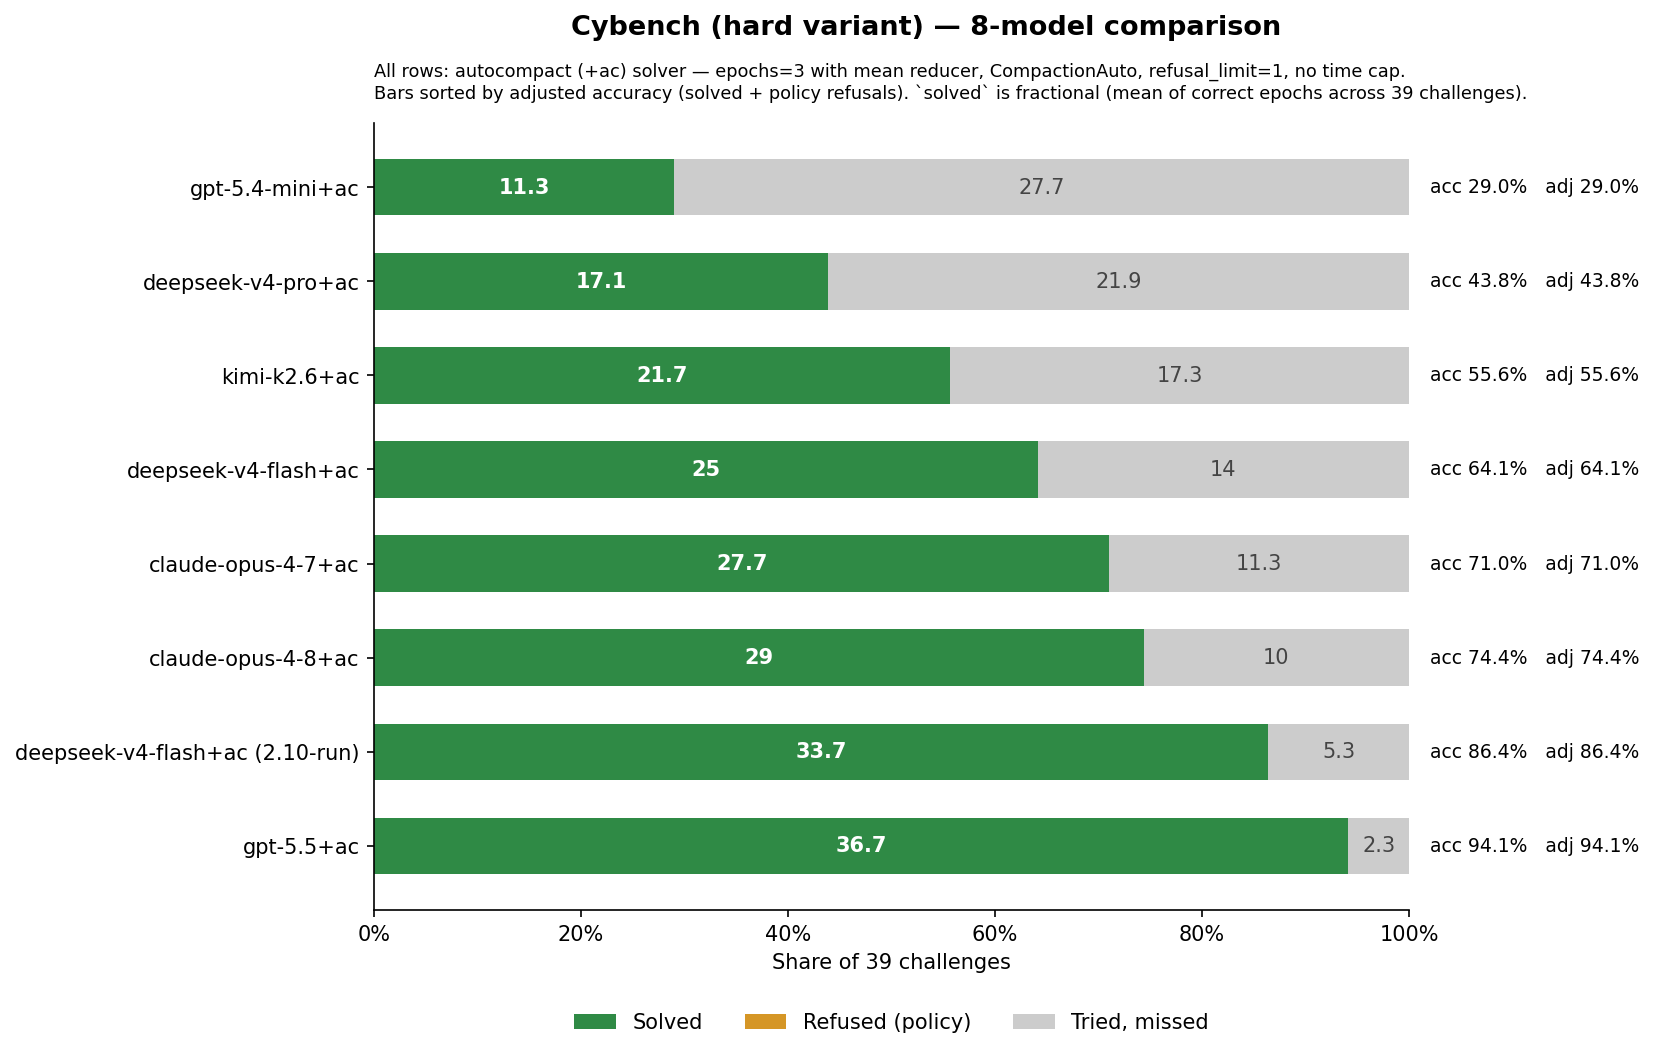
\includegraphics[width=0.95\linewidth]{cybench_comparison.png}
\end{center}
\noindent\textbf{Figure~\thefigure:} Cybench hard-variant comparison generated by source-repository \texttt{charts/make\_report.py}.
\par\medskip

\subsection{BOTSv1: public leaderboard scores require contamination controls}

Table~\ref{tab:bots} gives the BOTSv1 leaderboard.  Claude Opus 4.8 leads by BOTS points: 9,666.7 of 10,300 possible points (93.9\%), with 96.8\% binary accuracy.  It is also the most tool-efficient full run in the table: 603 total tool calls across 31 questions and three epochs.  A question-level paired bootstrap over the 31 scored questions puts Claude's margin over the standard GPT-5.5 row at +12.8 percentage points (95\% CI +0.9 to +27.4).  GPT-5.5 reaches about 81\% of points with 1,481--1,580 calls, while DeepSeek v4 Pro and Flash use still more calls and score lower.  Raising DeepSeek v4 Flash's cap from \$2.10 to \$4.20 adds only 91.7 points; its paired bootstrap interval crosses zero, so I treat that budget change as inconclusive rather than a meaningful gain.

\par\medskip
\refstepcounter{table}\label{tab:bots}
\noindent\textbf{Table~\thetable:} BOTSv1 full-run results from \texttt{charts/botsv1\_report.html}.  BOTS points are the primary \texttt{bots\_points} metric with hint penalties; binary accuracy is secondary.
\begin{center}
\resizebox{\linewidth}{!}{%
\begin{tabular}{lrrrrrrr}
\toprule
Model & BOTS points & points & binary acc. & model cost & tool cost & model+tools & tool calls \\
\midrule
Claude Opus 4.8 & 9{,}666.7 / 10{,}300 & 93.9\% & 96.8\% & \$11.81 & \$1.43 & \$13.24 & 603 \\
GPT-5.5 (high effort) & 8{,}383.3 / 10{,}300 & 81.4\% & 91.4\% & \$46.05 & \$2.94 & \$48.98 & 1{,}580 \\
GPT-5.5 & 8{,}345.0 / 10{,}300 & 81.0\% & 90.3\% & \$41.75 & \$5.54 & \$47.28 & 1{,}481 \\
DeepSeek v4 Pro & 8{,}013.3 / 10{,}300 & 77.8\% & 84.9\% & \$46.44 & \$0.48 & \$46.92 & 3{,}363 \\
DeepSeek v4 Flash (\$4.20 cap) & 7{,}610.0 / 10{,}300 & 73.9\% & 81.7\% & \$22.76 & \$0.53 & \$23.29 & 4{,}938 \\
DeepSeek v4 Flash & 7{,}518.3 / 10{,}300 & 73.0\% & 82.8\% & \$21.89 & \$0.64 & \$22.53 & 4{,}450 \\
GPT-5.4 Mini & 2{,}828.3 / 10{,}300 & 27.5\% & 41.9\% & \$18.16 & \$1.63 & \$19.79 & 1{,}693 \\
\bottomrule
\end{tabular}}
\end{center}

Because BOTSv1 is public and old, I ran a single-epoch no-tools probe using a memory-only solver.  No Splunk, web, bash, Python, or other tools were registered, and the logs contain zero tool events.  With the paper's prerequisite context enabled, Claude scored 7,700/10,300 points (74.8\%) and GPT-5.5 scored 6,400/10,300 (62.1\%).  With \texttt{prereq\_context=false}, Claude still scored 5,150 points (50.0\%) and GPT-5.5 scored 5,650 points (54.9\%).  These controls confirm substantial memorization or public-answer leakage; I therefore treat BOTSv1 as a useful harness and cost-accounting case study, not as clean evidence of fresh SOC investigation skill.

\par\medskip
\refstepcounter{figure}\label{fig:bots-decontamination}
\begin{center}
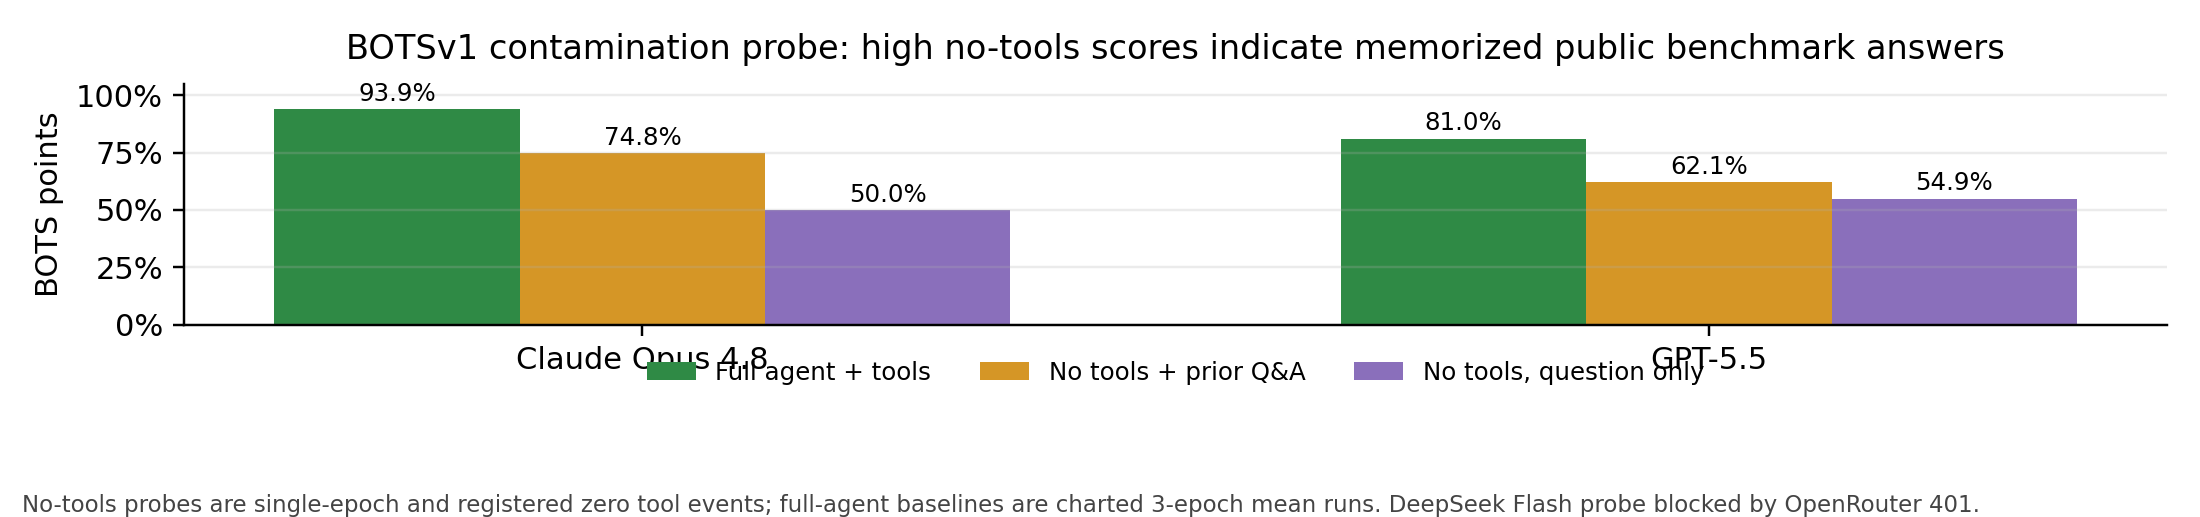
\includegraphics[width=0.95\linewidth]{botsv1_decontamination.png}
\end{center}
\noindent\textbf{Figure~\thefigure:} BOTSv1 no-tools contamination probe.  No-tools rows are single-epoch controls; full-agent baselines are charted three-epoch mean runs.  DeepSeek v4 Flash is omitted because OpenRouter authentication failed before any scored samples completed.
\par\medskip

\section{Discussion and Limitations}

\paragraph{Do not extrapolate SOC readiness from CTF results.}  Cybench is valuable because it measures autonomous challenge solving in realistic sandboxes, but its task shape is closer to offensive exploitation and reverse engineering than to SOC work.  BOTS asks for log-schema discovery, SPL query formulation, hypothesis pruning, external enrichment, and answer formatting under a point-and-hint economy.  The model ordering and resource behavior differ across these task families, so organizations selecting a model for security operations should evaluate on SOC-native workloads; for public SOC benchmarks, they should also run no-tools or perturbed-question controls.

\paragraph{Compute scaling and tool scaling differ by task family.}  The DeepSeek v4 Flash Cybench ablation is evidence that additional per-sample budget can unlock offensive solves.  The analogous BOTSv1 budget increase yields only a small point gain.  In these logs, full-agent defensive performance is associated less with brute-force tool volume than with targeted use of high-quality tools and evidence, but the no-tools controls show that this mechanism cannot be isolated cleanly on public BOTSv1 alone.

\paragraph{Cost accounting changes the question.}  In offensive CTFs, model-token spend is often the dominant marginal cost.  In SOC workflows, external data providers can be part of the real marginal cost of analysis.  Reporting model cost, tool cost, and combined cost makes this tradeoff visible, even though the values here exclude Kubernetes/Splunk infrastructure, free-tier effects, and any enterprise pricing variation.

\paragraph{Limitations.}  The experiments are not a randomized, controlled model-only benchmark.  Cybench rows differ in cost limits, routing, concurrency, sandbox backend, retry-chain cost ledgers, and one challenge-set denominator.  BOTSv1 rows are more uniform at the task level, but provider defaults and reasoning settings still differ.  Bootstrap intervals are descriptive robustness checks, not formal claims of population-level significance.  The defensive analysis covers BOTSv1 only; other SOC datasets and BOTS versions differ in scenario and operational maturity.  The no-tools probes confirm that BOTSv1 absolute scores are contamination-sensitive, and external-enrichment drift remains a separate threat to validity.

\section{Ethics, Artifacts, and Conclusion}

The experiments use public cybersecurity benchmarks and sandboxed environments.  The paper does not publish raw transcripts, secrets, API keys, or exploit instructions beyond high-level benchmark descriptions.  A sanitized supplement can provide aggregate provenance, uncertainty calculations, exact commands, commit hashes, model/provider identifiers, and cost-accounting details without releasing private logs or credentials.

The central finding is simple: security tasks should not be collapsed into one scalar capability.  Offensive CTF benchmarks and defensive SOC investigations stress different agent behaviors and show different scaling patterns, but public SOC benchmarks also need decontamination controls.  Evaluation programs should therefore report task-family-specific results, use scoring that matches the real workflow, account for model and external-tool costs, and test whether agents can answer without evidence tools.  For SOC adoption in particular, the right benchmark is not only ``can the model solve CTFs?'' but ``can the model investigate incidents like an analyst?''

\ifanonymousreview
\else
\section*{Acknowledgments}

Thanks to the maintainers of Inspect, Inspect Evals, Cybench, and Splunk's public BOTS datasets.
\fi

{\small
\bibliographystyle{plainnat}
\bibliography{references}
}

\end{document}
